\documentclass[12pt,a4paper]{report}
\usepackage{amsmath}
\usepackage{amsfonts}
\usepackage{amssymb}
\usepackage{graphicx}
\usepackage{multicol}
\usepackage[utf8]{inputenc}
\usepackage{array}
\usepackage{lipsum}
\graphicspath{{images/}}
\usepackage{parskip}
\usepackage{indentfirst}
\usepackage{courier}
\usepackage{titlesec}
\usepackage{wrapfig}
\usepackage{caption}
\usepackage[left=1.5in, right=1in, top = 1in, bottom = 1in]{geometry}
\usepackage{float}
\usepackage[ruled]{algorithm}
\usepackage{algpseudocode}
\usepackage{graphicx}
\usepackage{apacite}
\usepackage{url}
\usepackage{rotating}

\geometry{headheight = 12pt}
\parindent 15pt
\parskip 2ex

\usepackage{listings}
\usepackage{color}
\definecolor{lightgray}{rgb}{.9,.9,.9}
\definecolor{darkgray}{rgb}{.4,.4,.4}
\definecolor{purple}{rgb}{0.65, 0.12, 0.82}

\lstdefinelanguage{JavaScript}{
	keywords={typeof, new, true, false, catch, function, return, null, catch, switch, var, if, in, while, do, else, case, break},
	keywordstyle=\color{blue}\bfseries,
	ndkeywords={class, export, boolean, throw, implements, import, this},
	ndkeywordstyle=\color{darkgray}\bfseries,
	identifierstyle=\color{black},
	sensitive=false,
	comment=[l]{//},
	morecomment=[s]{/*}{*/},
	commentstyle=\color{purple}\ttfamily,
	stringstyle=\color{red}\ttfamily,
	morestring=[b]',
	morestring=[b]"
}

\lstset{
	language=JavaScript,
	backgroundcolor=\color{lightgray},
	extendedchars=true,
	basicstyle=\footnotesize\ttfamily,
	showstringspaces=false,
	showspaces=false,
	numbers=left,
	numberstyle=\footnotesize,
	numbersep=9pt,
	tabsize=2,
	breaklines=true,
	showtabs=false,
	captionpos=b
}

\algblockdefx[ClassBlock]{Class}{EndClass} [1]{\textbf{class} #1} [0]{}
\algtext*{EndClass}

\newcommand{\WRP}{\par\qquad\(\hookrightarrow\)\enspace}

\renewcommand{\listfigurename}{Figures}
\renewcommand{\listtablename}{Tables}

\titleformat{\chapter}[display]   
{\normalfont\huge\bfseries}{\chaptertitlename\ \thechapter}{20pt}{\Huge}   
\titlespacing*{\chapter}{0pt}{-50pt}{20pt}

\author{Group 42 \\ -------------------- \\Jacob Spigle, Zachary Painter, David Akridge, Hunter Figueroa}
\title{Critical Encounters}
\begin{document}
	
\maketitle

\tableofcontents
	
\newpage
\chapter*{Introduction}
\stepcounter{chapter}
\addcontentsline{toc}{chapter}{Introduction}

Role-playing games are games where players act as their characters. Usually in person, around a table, and controlled by the players speaking their actions in turn. This might not always be done by speaking in-character, but rather by following this basic structure:

\begin{enumerate}
	\item The GM describes the environment.
	\item The players describe what they want to do.
	\item The GM narrates the results of the characters? actions.
\end{enumerate}

There are countless possible character, monster, and scenario possibilities when constructing a tabletop role-playing campaign, however, it is hard and sometimes impossible to sift through them all and find the perfect encounter. Not only that,  but once you commit to a game or role-playing decision you are forced to see it through to completion in order to retain the game?s continuity. Players get one chance to design their character at the very start of a session, and once they do, that character?s path cannot be meaningfully changed. Spending so much time working on a character, and then coming to the first session to find out that they are severely unprepared for the tasks they are presented can be harrowing. On the other side, the GM spends so much time outside of the game to prepare a story and encounters that challenge the Players, so when that GM accidentally wipes out the entire team of Player Characters (PCs) in one unbalanced encounter, or if the PCs simply walk through a fight that was meant to challenge them for the remainder of the session, the GM feels they have failed the PCs in presenting a good game.
\newpage
\chapter*{Proposed Solution}
\stepcounter{chapter}
\addcontentsline{toc}{chapter}{Proposed Solution}

This project presents a service that can be used by both GMs and players to test out their characters, encounters, team builds, or boss fights in a simulated environment. This will allow users to figure out just how well their creation holds up to the requirements that they have set for themselves, and perfect them to ensure the most enjoyable experience in a live game encounter.

This project seeks to develop a service that allows a user to create an encounter that follows the rules of the d20 Game System. The creator streamlines the refining process by easily being able to simulate the encounter. By allowing the player or GM to import their character's/monsters' statistics and equipment, they then can play against an automated opponent or opponents using that creation. The encounters will have the ability to be rapidly simulated over and over to display statistics about the encounter the help improve the encounter. To further enhance a user's ability to test and refine encounters and PCs, users will be able to upload and share their encounters to their public space where others can try their own creations' skills in that creator's setting.

\newpage
\chapter*{Broader Impact}
\stepcounter{chapter}
\addcontentsline{toc}{chapter}{Broader Impact}

Tabletop games bring people together in a world where physical interaction is often lost in lieu of digital communication. This project aims to supplement these interactions by making them more accessible to newer players, as well as help experienced players spend less time on pre-game preparation. In-game encounters require large amounts of time to plan, setup, and implement, so by enhancing this process and giving the GM the ability to perfect an encounter beforehand the whole process becomes more enjoyable for anyone playing the game.

This project has the potential to broaden the audience of an already quickly expanding pastime to younger players and DM's. Concepts in the realm of tabletop games are very easily understood by a younger audience, as their imagination and creativity can run free in such games. However, the threshold of understanding for the many rules and balances may prove a bit overzealous for this audience. Having a service that allows improves accessibility to newer players will also bleed into improving accessibility for younger players as well. Additionally, users who do not have a group to play with may find and form groups with other users with whom they have played and shared content with.
	
\newpage
\chapter*{Personal Interests}
\stepcounter{chapter}
\addcontentsline{toc}{chapter}{Personal Interests}
	\section{Jacob Spigle}
	\begin{wrapfigure}{r}{0\textwidth}
		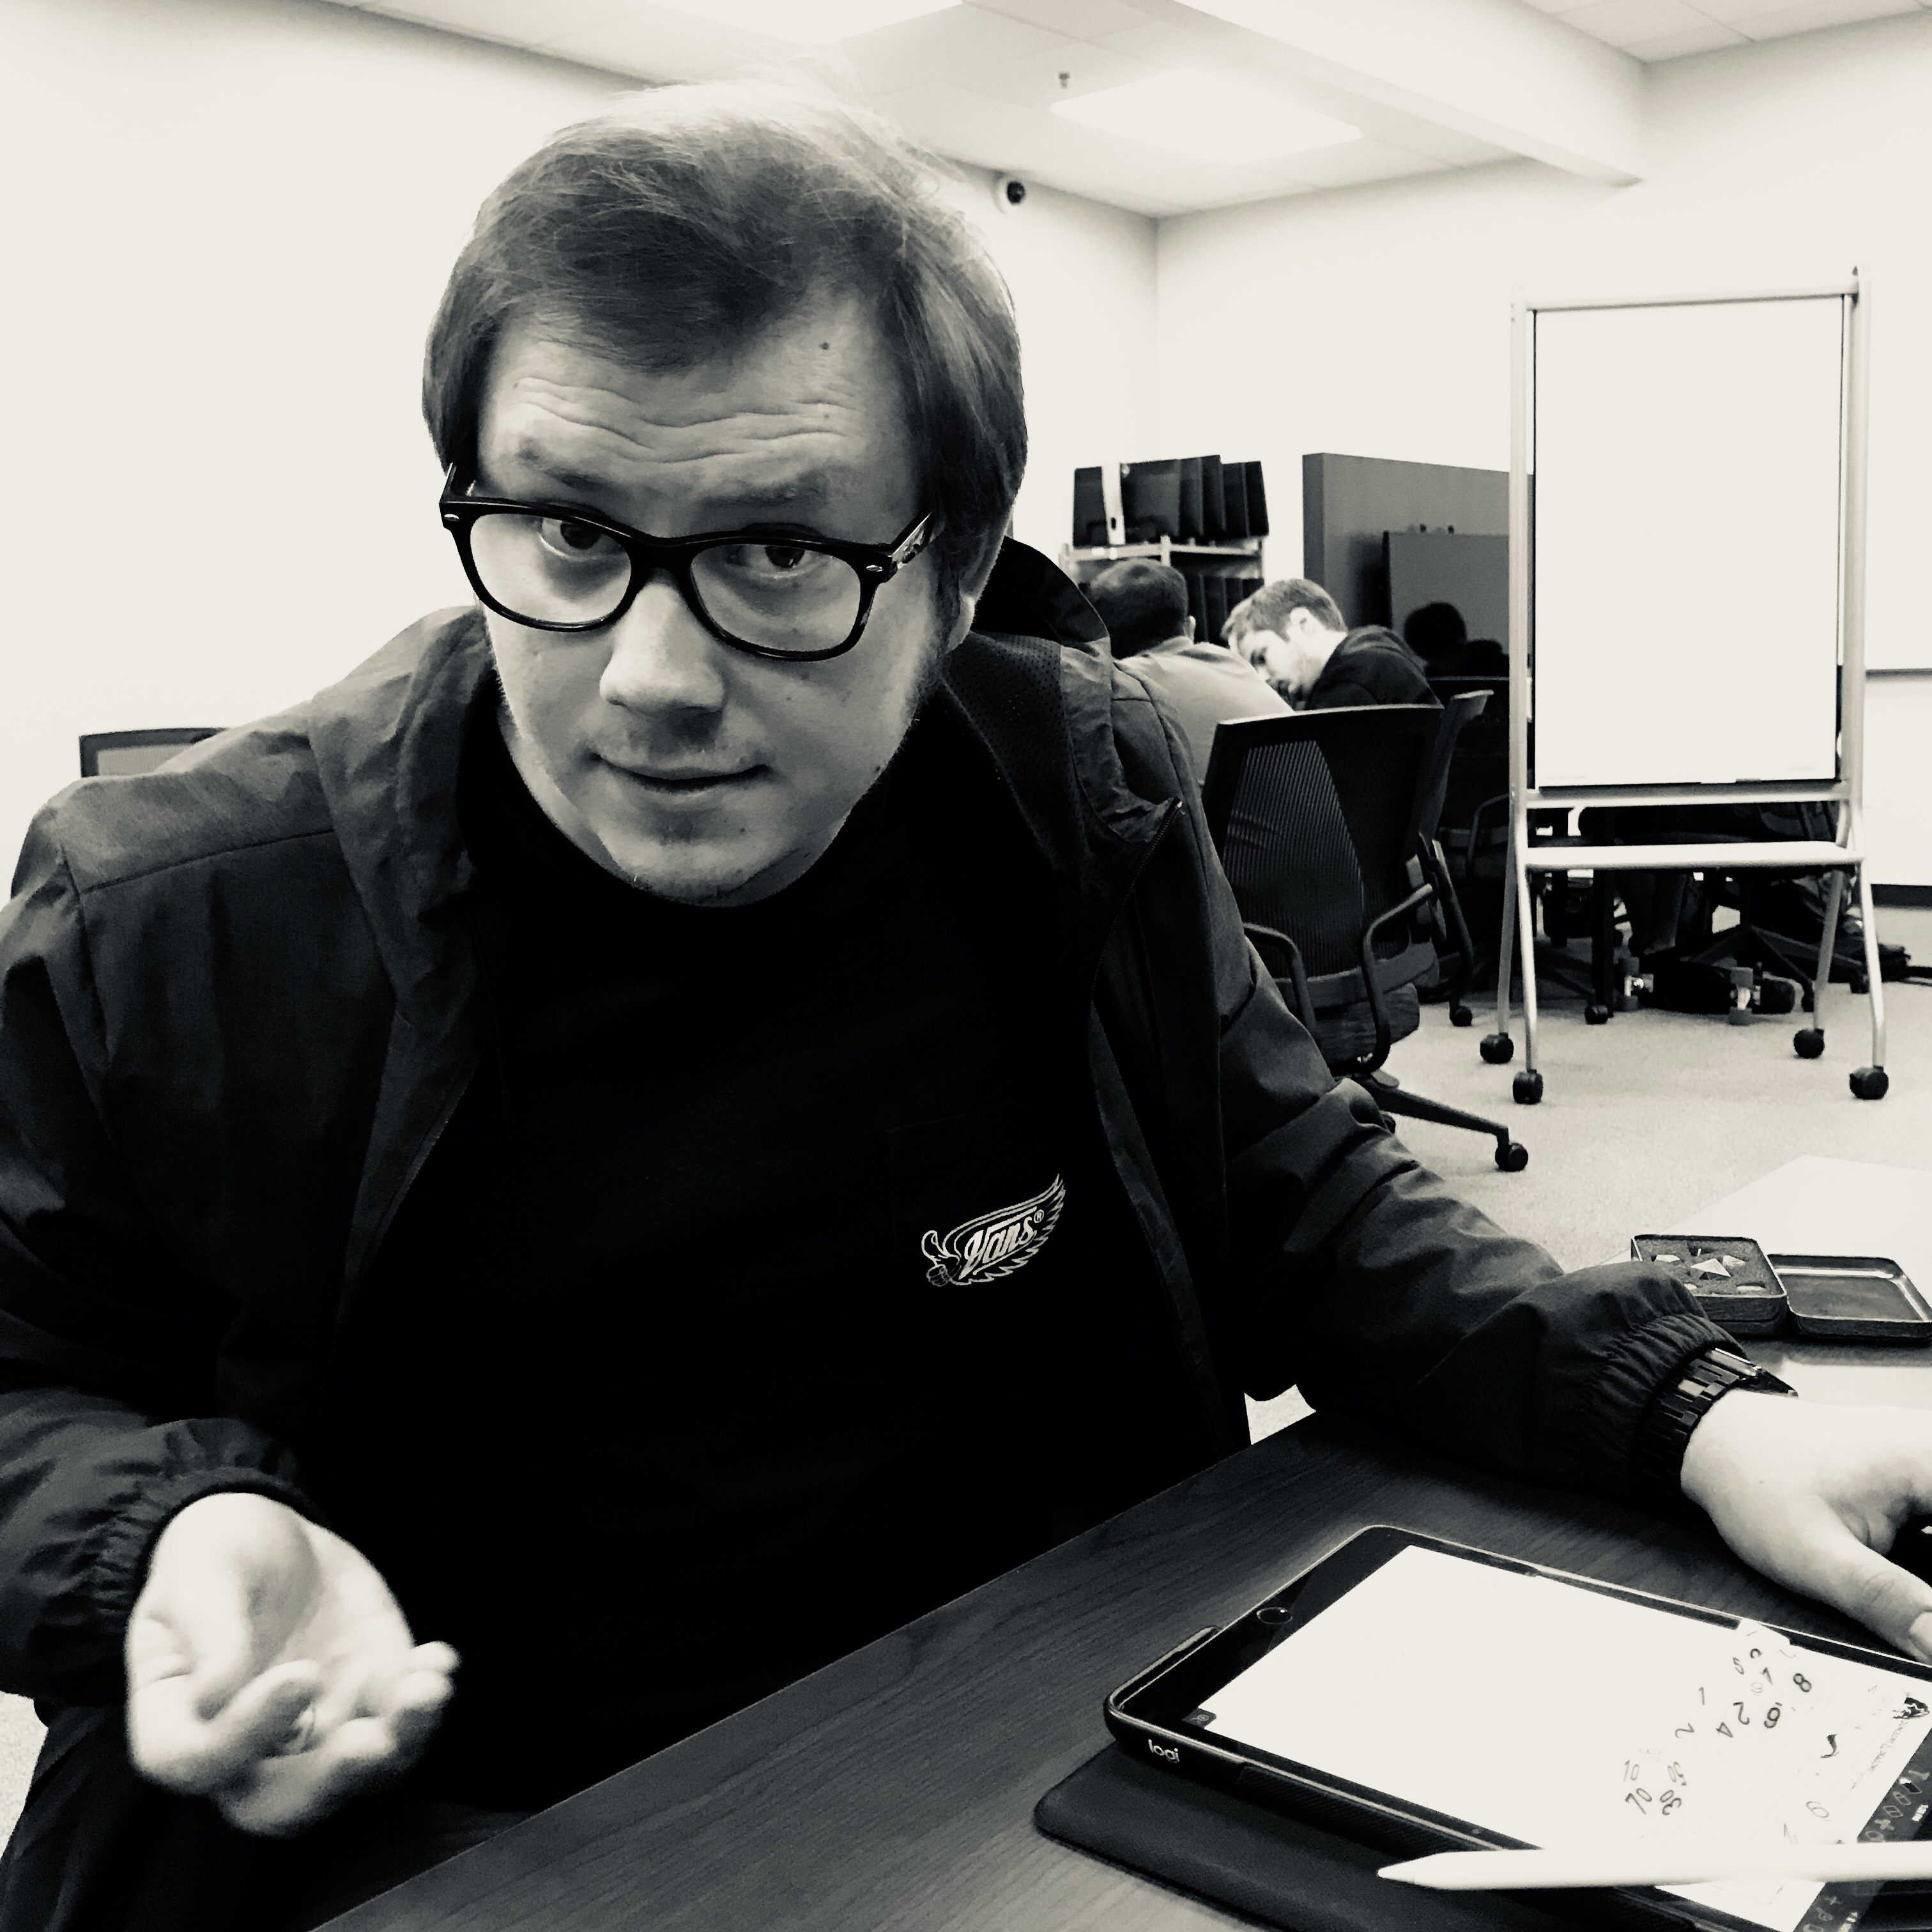
\includegraphics[scale=0.05]{Jacob_Spigle}
	\end{wrapfigure}
	I discovered role-playing games like Dungeons \& Dragons early this year. After playing video games since childhood, D\&D was a breath of fresh air; a way to mix the excitement of creating a character, leveling up, deciding your actions, along with an openness that allows nearly infinite stories, infinite worlds, and the tools to create those stories and worlds yourself. Those infinite possibilities can spur creations that might not work as well in-game as you thought. I have written campaigns and characters that on paper seemed great, but when brought to the table were found lacking. When I searched through the many different forums and groups I had joined after I started playing D\&D, and scouring the internet for a way to playtest my creations, I was surprised to found that no such tool existed. This service is something I can actually use and wish that I had during the creation of campaigns I have written, and that is why I believe others will find use in it as well.
	
	\newpage
	\section{Zachary Painter}
	\begin{wrapfigure}{l}{0\textwidth}
		
\includegraphics[scale=0.05]{Zachary_Painter}
	\end{wrapfigure}
	Some of my primary interests in Computer Science are data structures and algorithms. In my area of research, concurrent programming, these two topics are frequently discussed. Often times in this field, I have had the opportunity to explore many complicated and fascinating algorithms. When tackling these kinds of problems, you often find yourself spending considerably more time thinking and reasoning than implementing/coding. After understanding a problem, you move on to another without getting the chance to apply what you learned in a practical/usable way. This constant cycle of struggle/learn/get-new-problem is something that many students experience throughout college as they rarely have time to stop and demonstrate their rapidly growing skillset in a meaningful way. \par
	My motivation for being part of this project is that I want a chance to slow down and use the skills and algorithms I have picked up in my years at UCF in a useful and creative application instead of an abstract, un-impactful thought exercise. Instead of expecting this project to challenge me with highly complicated algorithms and difficult proofs, I expect this project to challenge me in project management skills, team coding, and the application of numerous techniques that I have learned but never had to implement in a meaningful way. There is an important difference between \textit{knowing} and \textit{doing}; and so I am taking this chance to remind myself what all my learning has amounted to. 
	
	\newpage
	\section{David Akridge}
	\begin{wrapfigure}{r}{0\textwidth}
		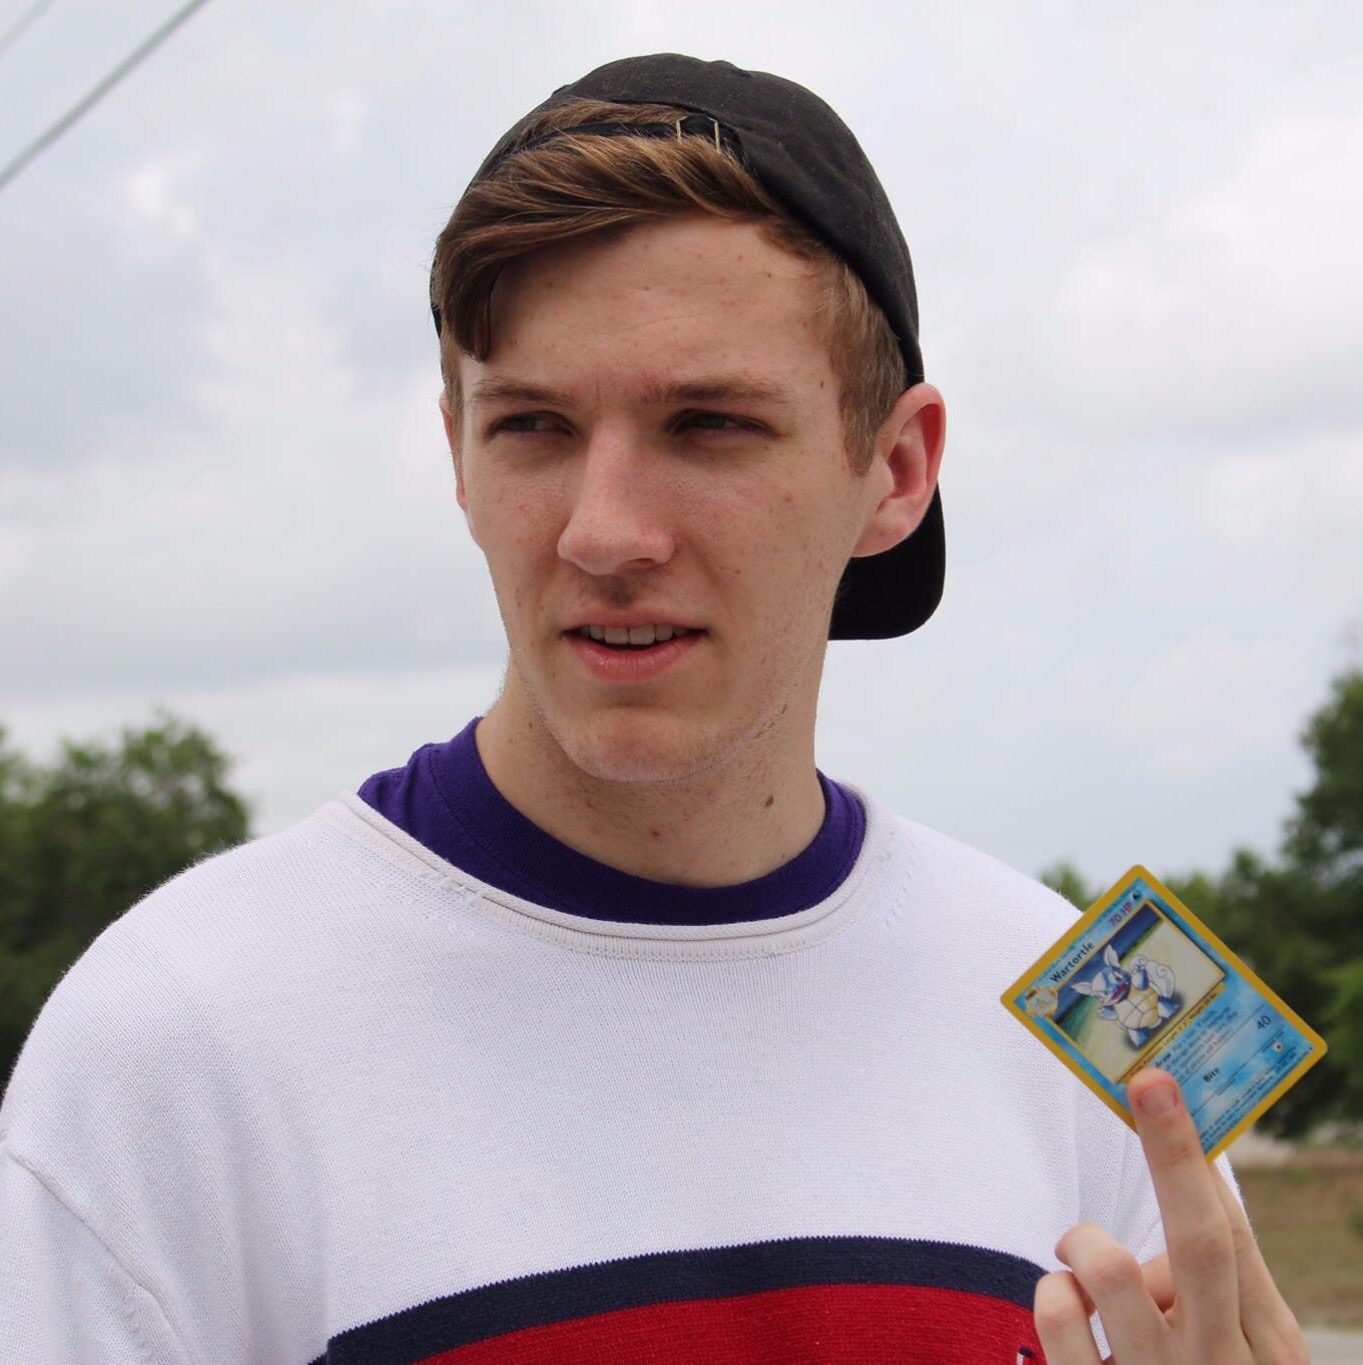
\includegraphics[scale=0.05]{David_Akridge}
	\end{wrapfigure}
	This project caught my interest due to the combination of the creative nature of Dungeons \& Dragons mixed with the real world applications that can be gained by accomplishing the project’s end goal. In my time at UCF, we have learned tons of information primarily focusing on theories and concepts of computer science. While plenty of classes have had us working hands on, there is still much to learn before being able to stand out in the real world. This project is going to have us utilize the various algorithm implementations we’ve learned as well as diving into web development. As we haven’t covered web development in too far detail in the UCF curriculum, this project easily provides an opportunity for me to grasp the understanding of HTML, Javascript, Angular.js, etc. These are all languages and formats that I have had the desire the learn but lacked the drive to do on my own. \par
	Along with being able to learn practical CS skills, Critical Encounters will allow us to find creative workarounds be it code, web-page design, or even artwork. This is a really important aspect of the project to me, because many of the projects we’ve had to do prior have been numerically heavy and honestly not all that interesting. An engaging idea could help propel our ability to learn these new concepts, especially if we are interested in them on our own. Now that there is a great project motivating me and a great team to work alongside with, there is no doubt we will learn all the in’s and out’s of the subject. 
	
	\newpage
	\section{Hunter Figueroa}
	\begin{wrapfigure}{l}{0\textwidth}
		
\includegraphics[scale=0.05]{Hunter_Figueroa}
	\end{wrapfigure}
	I have been playing tabletop role-playing games for over 6 years now. They served as a creative outlet where I could experiment with new creative ideas. I prefer acting as a DM, I’ve only played a single session as a player, I loved the idea of being all powerful creator of a world that I could share with my friends. The tabletop community, namely the Dungeon \& Dragons community is like no other that I have seen before. It is composed of highly talented, highly cooperative  and interactive people who do their very best to better and expand the role playing community. For close to two years now I have put a considerable about of my free time into constructing a digital service to help this same cause. So when I heard Jacob pitch this idea, I knew it was the one for me. We’ve got something really special here, and with the team that we have I feel we can create something game changing.
	
\newpage
\chapter*{User Interface}
\stepcounter{chapter}
\addcontentsline{toc}{chapter}{User Interface}
	\section{Overall Design and Navigation Bar}
	The approach we took to user interface (UI) design was focused on a simplistic and familiar look and feel to allow for easy accessibility to new users while the website itself still retaining focus on the encounter tester. The template that website utilizes is reminiscent of the design that many social media sites take, for instance, sites like Twitter, Facebook, and YouTube.\par
	The site also uses the the single-page application structure that allows for easy traversal. The persistent navigation bar (Figure \ref{fig: NavBar}) has Critical Encounters' name and logo in the top left of each page which redirects users back to the homepage, a searchbar in the top of each page which redirects users to the Encounter Browser page, and the user's username in the top right of each page that links to the user's Arena.
	\bigskip
	\bigskip
	\begin{figure}[H]
		\centering
		\centerline{
\includegraphics[scale=.30]{navbar}}
		\caption{NavBar}
		\label{fig: NavBar}
	\end{figure}
	\section{Registration Page}
	\begin{figure}[H]
		\centering
		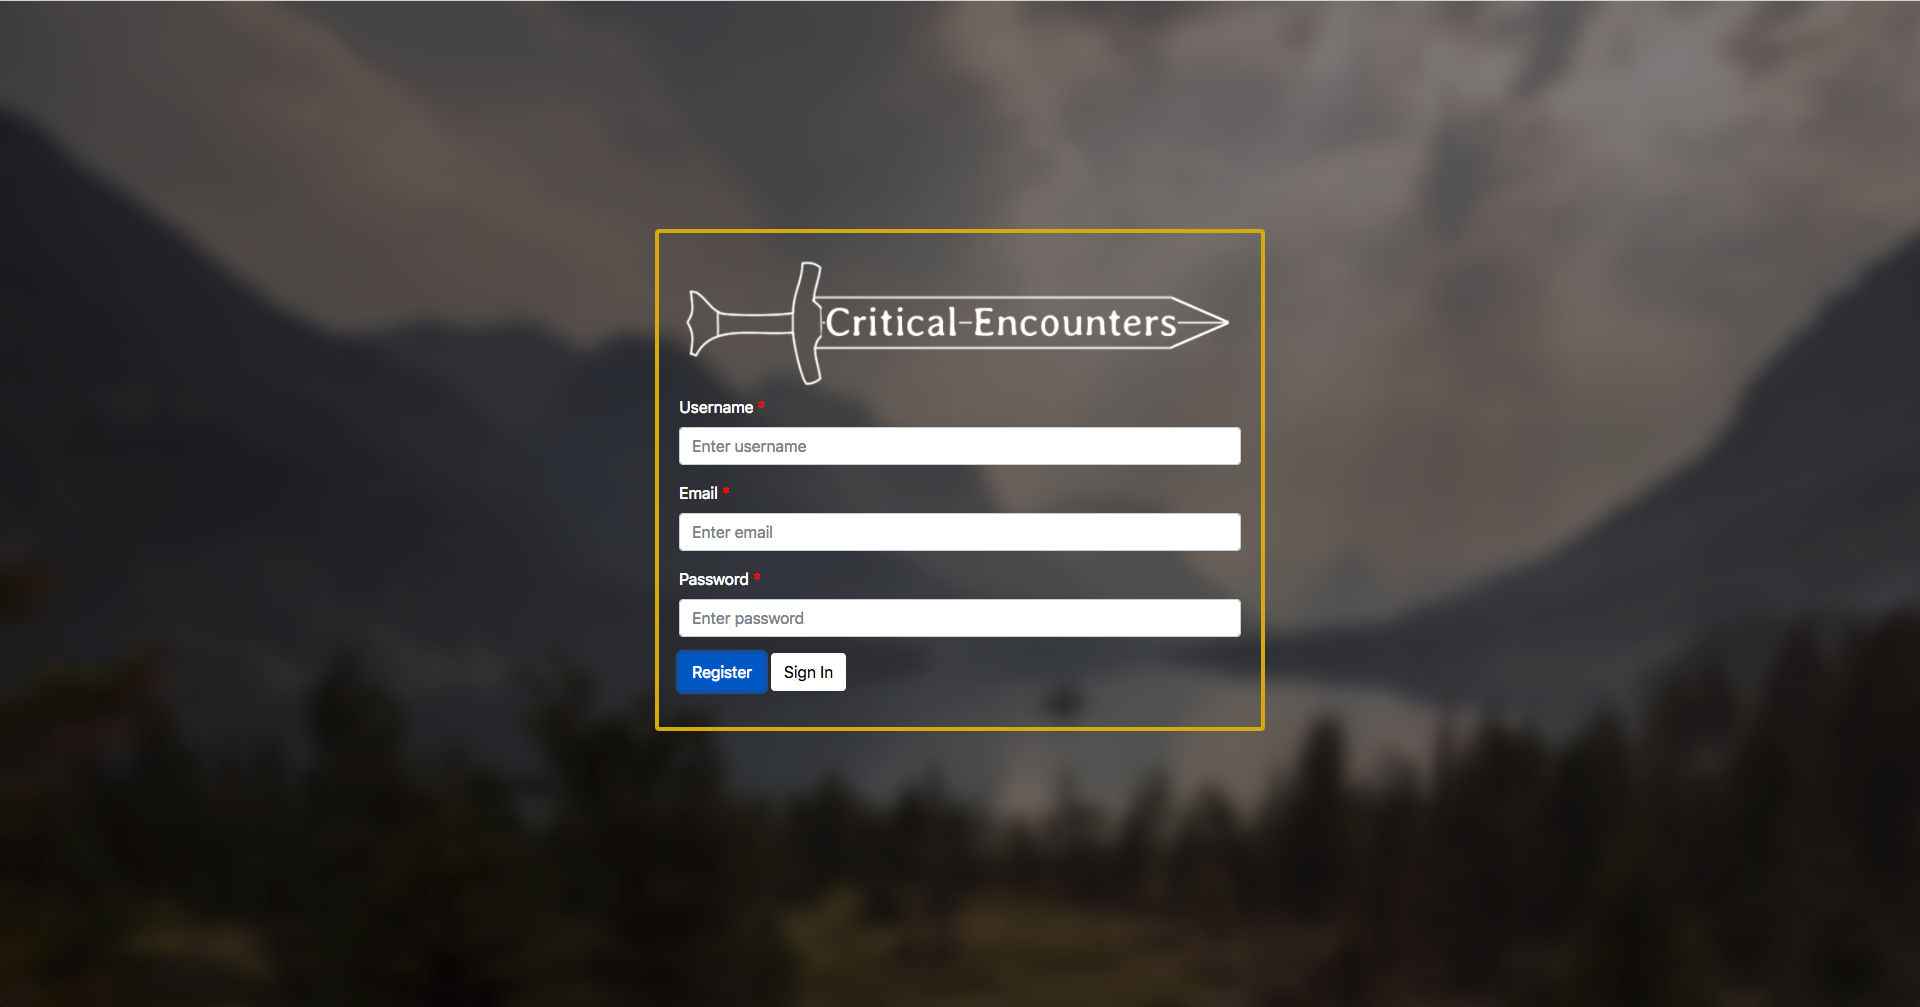
\includegraphics[scale=.20]{register}
		\caption{Registration Page}
		\label{fig: Registration Page}
	\end{figure}
	The registration page (Figure \ref{fig: Registration Page})  for Critical Encounters requires the user's desired username, their email address, and their password. Users are directed to the registration page from the Dashboard or from clicking the ``Register" link on the login page.
	\newpage
	\section{Login Page}
	\begin{figure}[H]
		\centering
		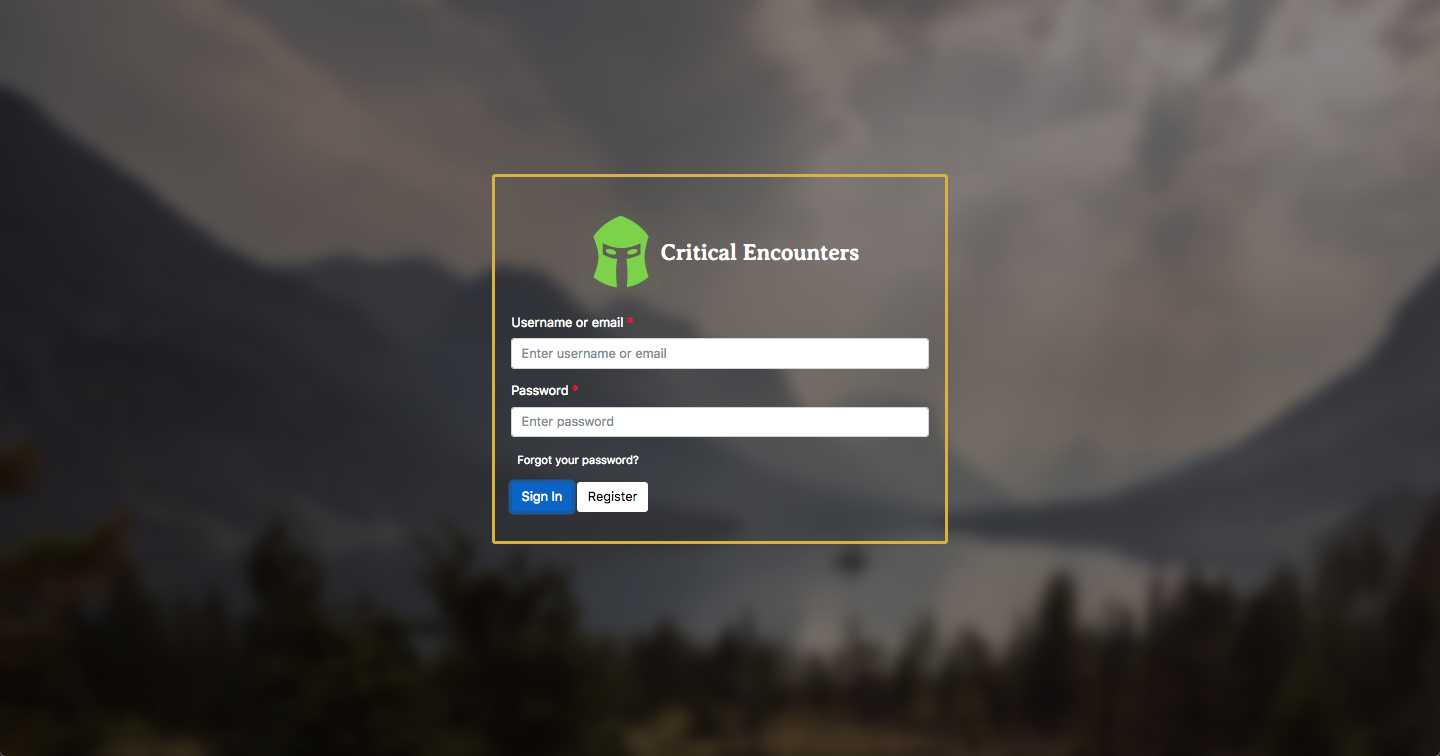
\includegraphics[scale=.20]{login}
		\caption{Login Page}
		\label{fig: Login Page}
	\end{figure}
	The login page (Figure \ref{fig: Login Page}) for Critical Encounters prompts users for their credentials to log in. Beneath the username/email address \& password fields is a ``Register" link to the registration page and a ``Forgot Password?" to a password retrieval service. Users are directed to the login page by clicking the ``Login" link on the navbar, or after attempting to access content that requires an account. (i.e. accessing the Battlefield, Arena, subscribing, reviewing, etc.)
	\newpage
	\section{Dashboard}
	\begin{figure}[H]
		\centering
		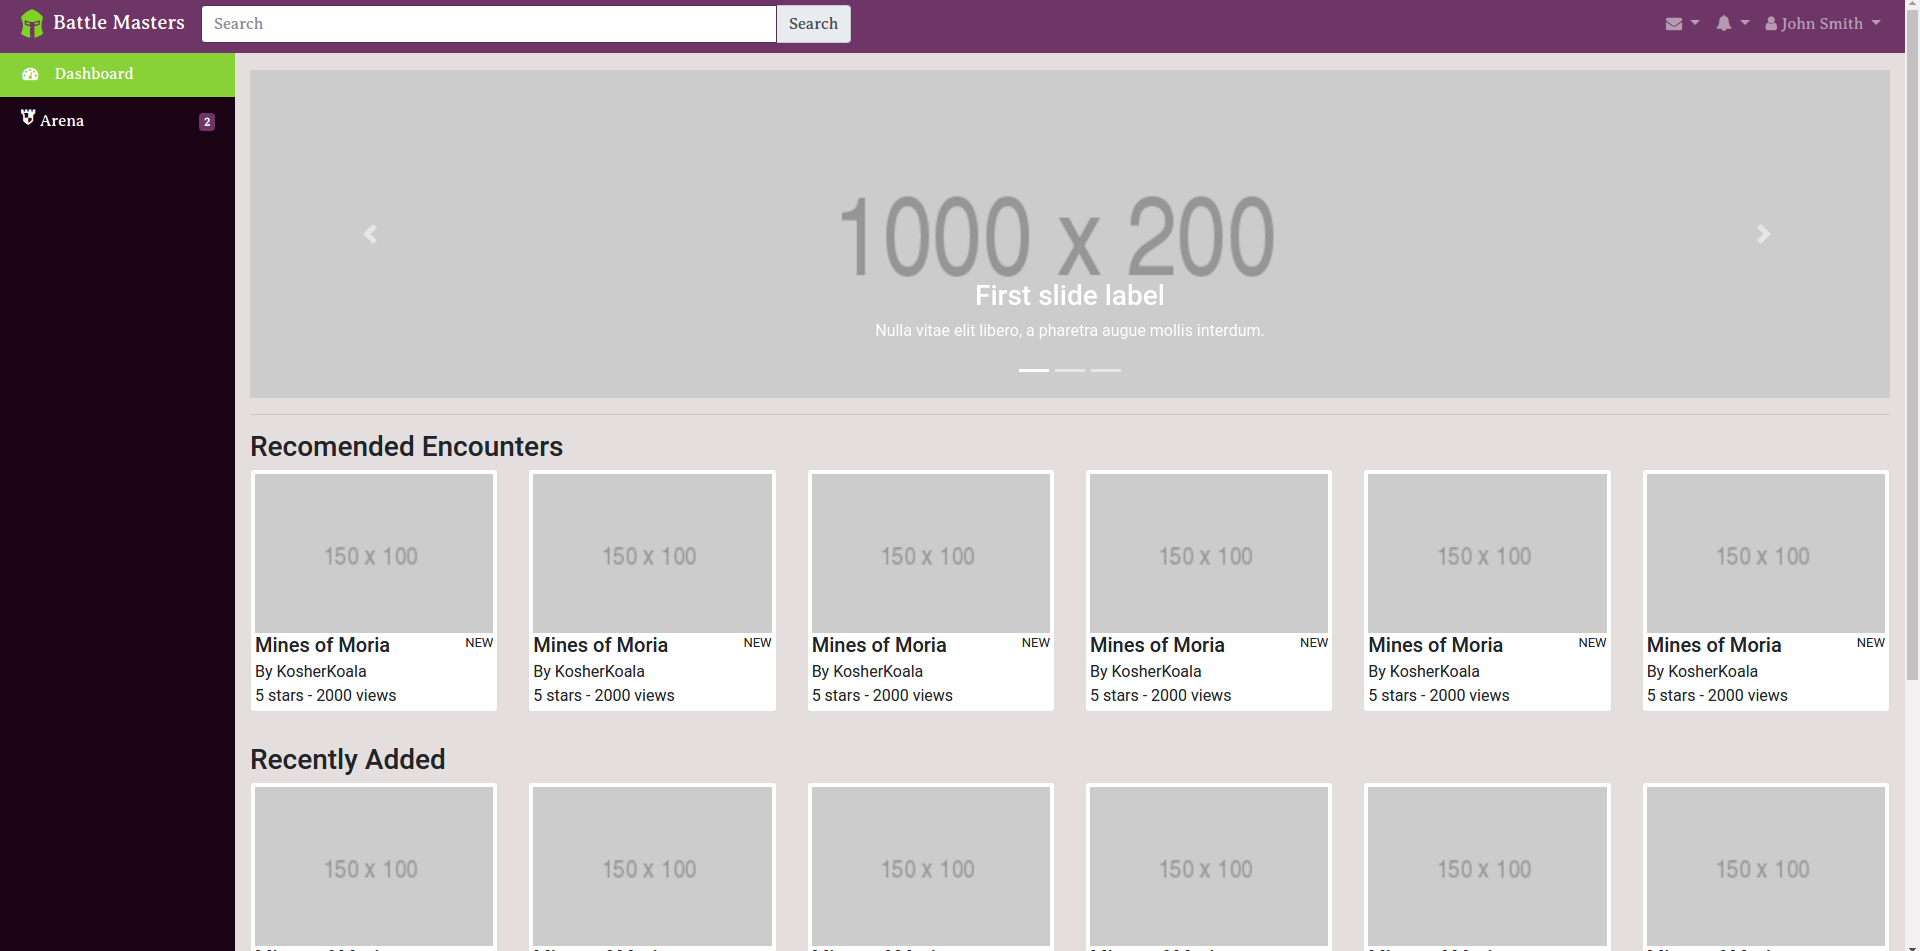
\includegraphics[scale=.20]{home}
		\caption{Dashboard}
		\label{fig: Dashboard}
	\end{figure}
	The Critical Encounters' Dashboard (Figure \ref{fig: Dashboard})features notable encounters, updates, and community events in the highlight wheel at the forefront of the page. Below the highlight wheel is a list of recommended encounters that either we the developers suggest to the community, or recommended list that is influenced by the user's recent search history.\par
	The Dashboard doubles as a homepage for the Critical Encounters website. Upon arrival on the site unregistered users will be directed to the Dashboard, with the highlight wheel, recommended encounters, etc. presented to them the same as a logged in user would see it. Clicking the ``Register" link on the navbar will bring the unregistered user to the Registration page, and The Arena link on the sidebar will do the same. 
	\newpage
	\section{Encounter Browser}
	\begin{figure}[H]
		\centering
		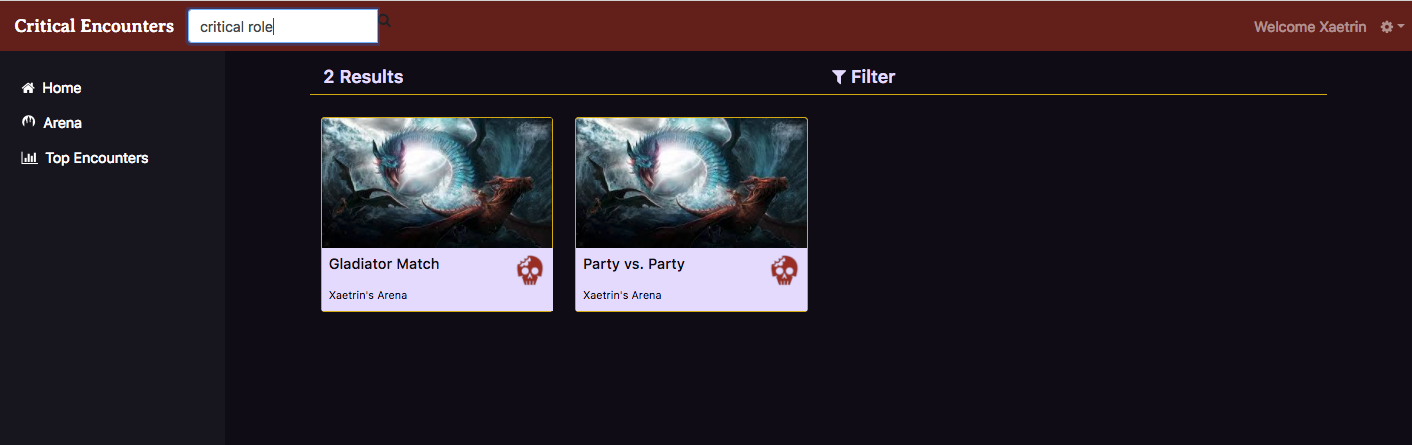
\includegraphics[scale=.19]{search}
		\caption{Encounter Browser}
		\label{fig: Encounter Browser}
	\end{figure}
	The Critical Encounters' Encounter Browser (Figure \ref{fig: Encounter Browser})acts as a search results page for queries entered in the search bar. From this page a list of filtered encounters is presented to the user. The user may also filter those results further by selecting settings from the dropdown menu revealed by the 'Filter' button. Through this process we can be sure to provide users with encounters that help with creation or spark their own imagination. (Figure \ref{fig: Encounter Browser with Filter Options}).
	\begin{figure}[H]
		\centering
		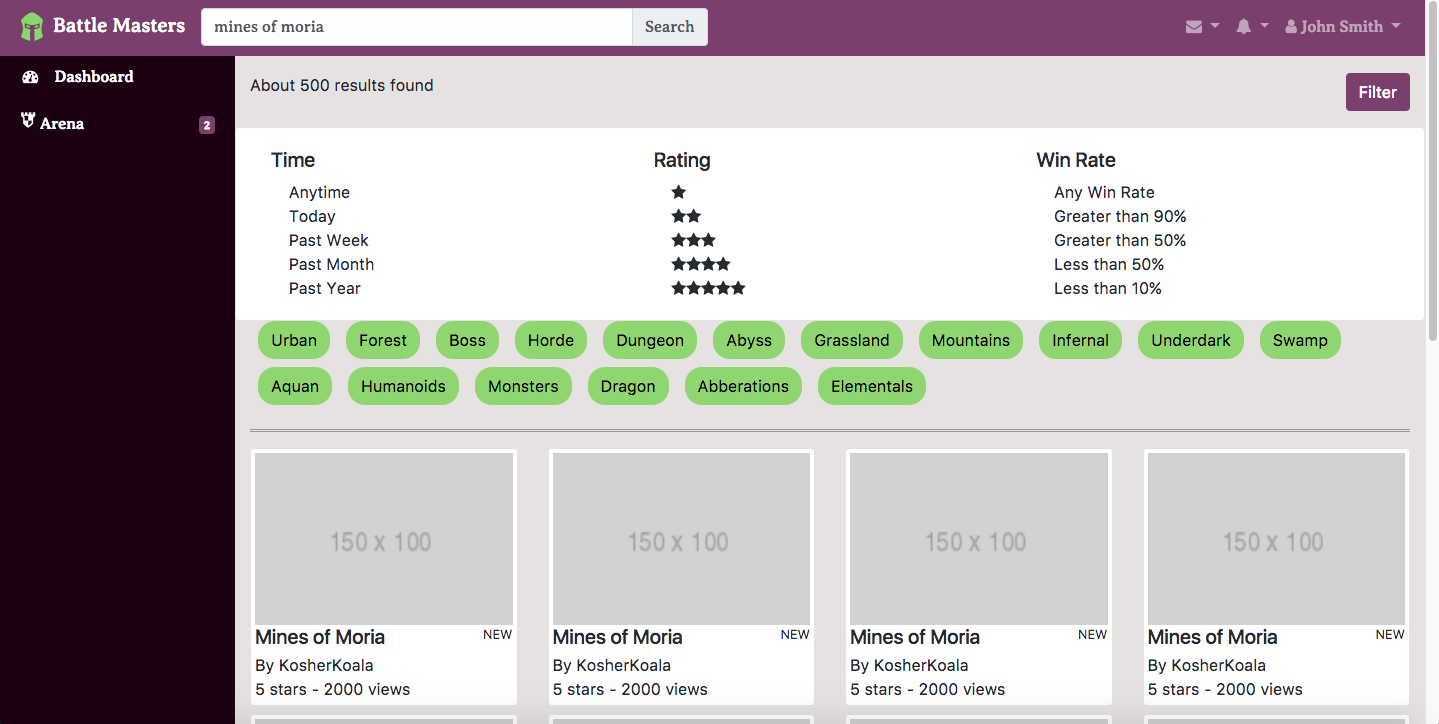
\includegraphics[scale=.25]{search_filtered}
		\caption{Encounter Browser with Filter Options}
		\label{fig: Encounter Browser with Filter Options}	
	\end{figure}
	\newpage
	\section{Arena}
	\begin{figure}[H]
		\centering
		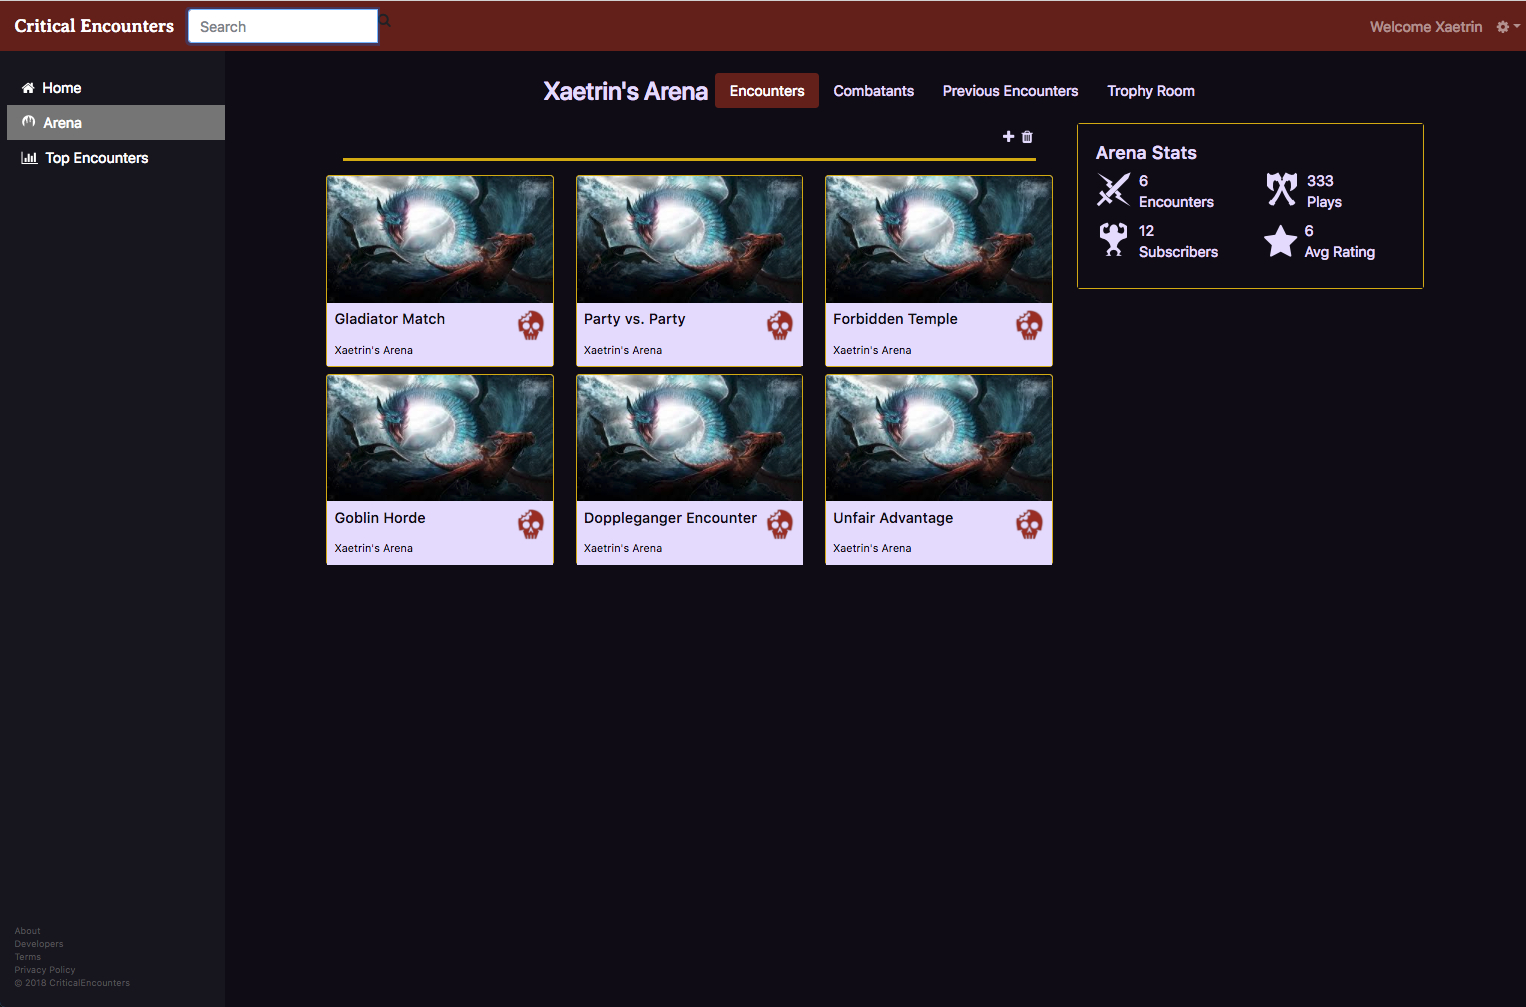
\includegraphics[scale=.20]{arena}
		\caption{Arena}
		\label{fig: Arena}
	\end{figure}
	Each Critical Encounters user is provided a page to host their published encounters for the rest of the community to access, their Arena. From the Arena page (Figure \ref{fig: Arena}) is where users are redirected to encounter creation within the Battlefield by clicking the ``Create Encounter'' button on their own Arena. Users also have the ability to edit their Arena, listing their created encounters in whatever order they wish, whether done manually or by analytics (Plays, Win Rate, Rating). At the top of the Arena page is the username and profile picture of the user tied to the Arena. The Arena presents the user's creations in a list format, with pertinent information listed alongside each encounter. Number of plays, PC win rate, overall rating, and the number of comments are shown under the encounter's title and description, and to the right of a screenshot or preset image of the encounter board itself. To the right of the encounter list, additional data on the user's arena is supplied: 
	\begin{multicols}{2}
		\begin{itemize}
			\item Number of Encounters
			\item Number of Subscribers
			\item Number of Plays
			\item Average Encounter Rating
		\end{itemize}
	\end{multicols}
	\noindent Below that, a graph illustrates each class' Win/Loss stats in the Arena.
	\newpage
	\section{Encounter Page}
	\begin{figure}[H]
		\centering
		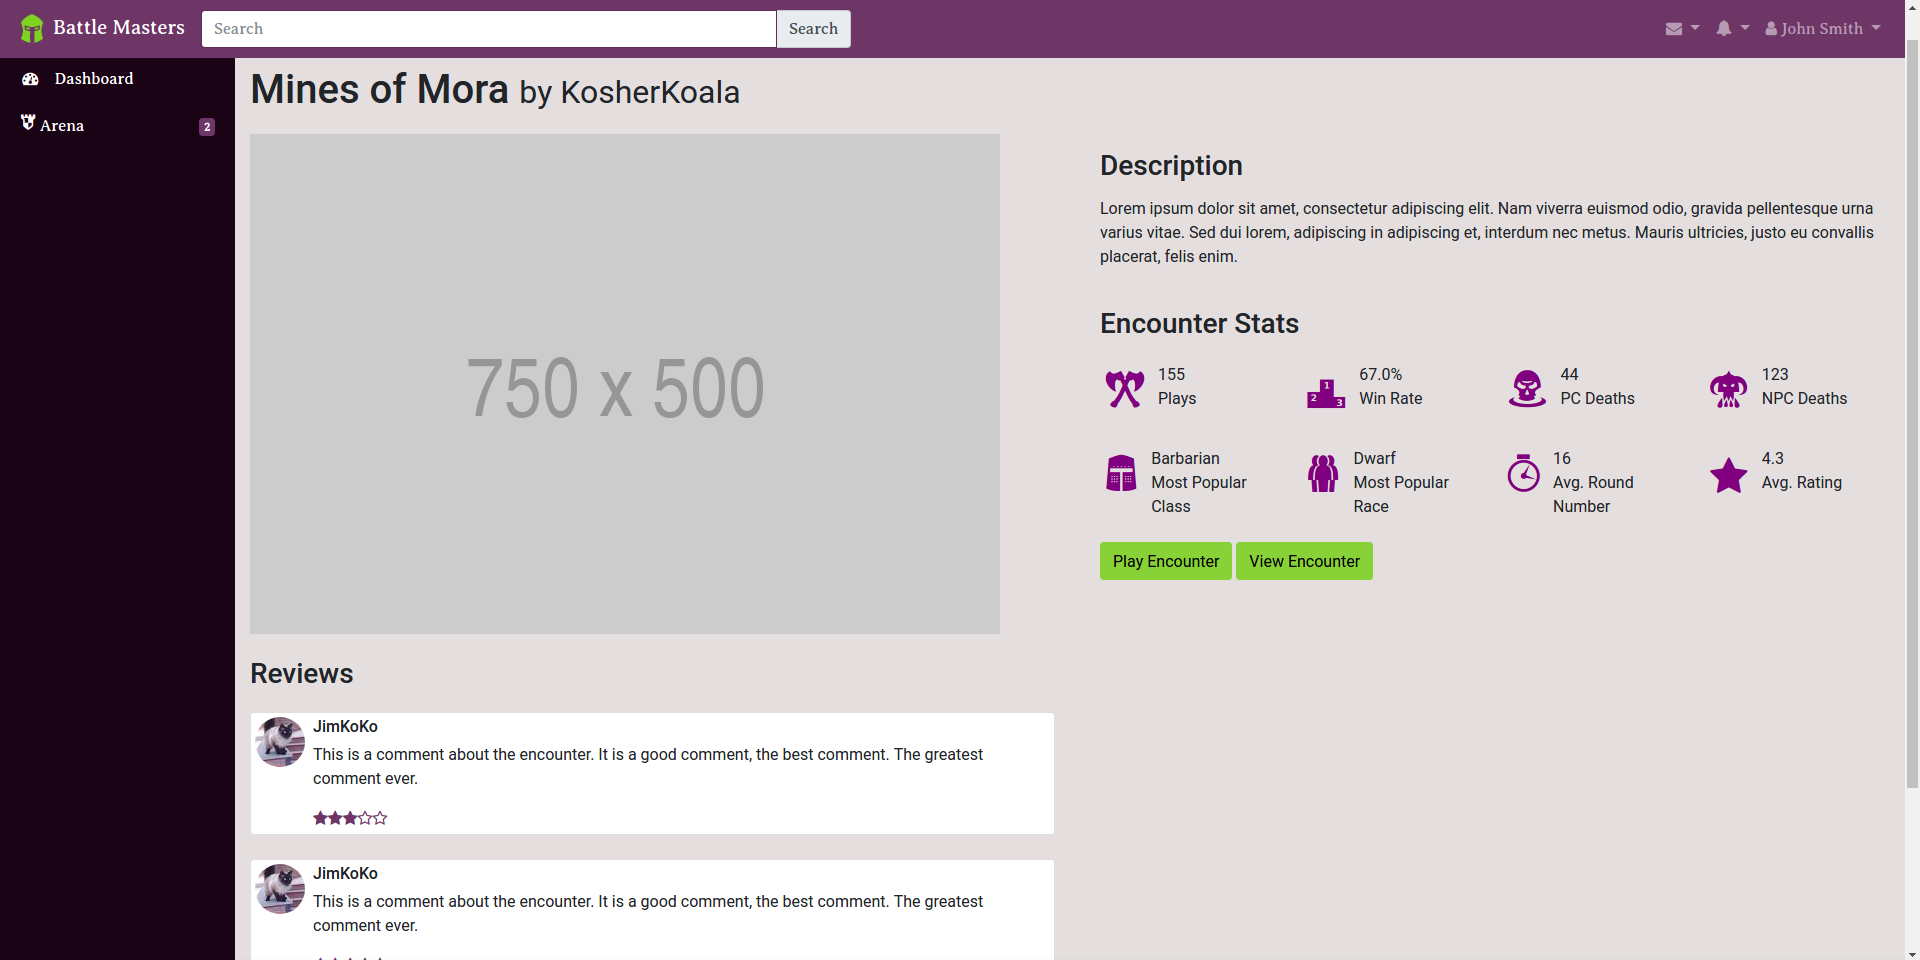
\includegraphics[scale=.20]{encounter}
		\caption{Encounter Page}
		\label{fig: Encounter Page}
	\end{figure}
	Each encounter created in Critical Encounter is given an encounter page, from which user's navigate to in order to start playing the encounter. At the top of the encounter page is the encounter's name, followed by the username of its' creator. Below is a screenshot or preset image of the encounter board, and the creator's description of the encounter hangs to the left of the image. The encounter page also presents the user with statistics related to the encounter:
	\begin{multicols}{2}
		\begin{itemize}
			\item Number of Plays
			\item Win Rate
			\item Number of PC Deaths
			\item Number of NPC Deaths
			\item Most Popular Class
			\item Most Popular Race
			\item Average Number of Rounds
			\item Average Rating
		\end{itemize}
	\end{multicols}
	\newpage
	\section{Battlefield}
The Battlefield is arguably the most important and most challenging frontend development we must complete. The Battlefield is where users will create, edit, and play their encounters. Because of its importance we have put a lot of thought into the requirements, design, and implementation plans. Both the frontend and backend are working closely on this component because the battlefield is the stage that our AI will be able to show its capabilities.
\begin{figure}[H]
	\centering
	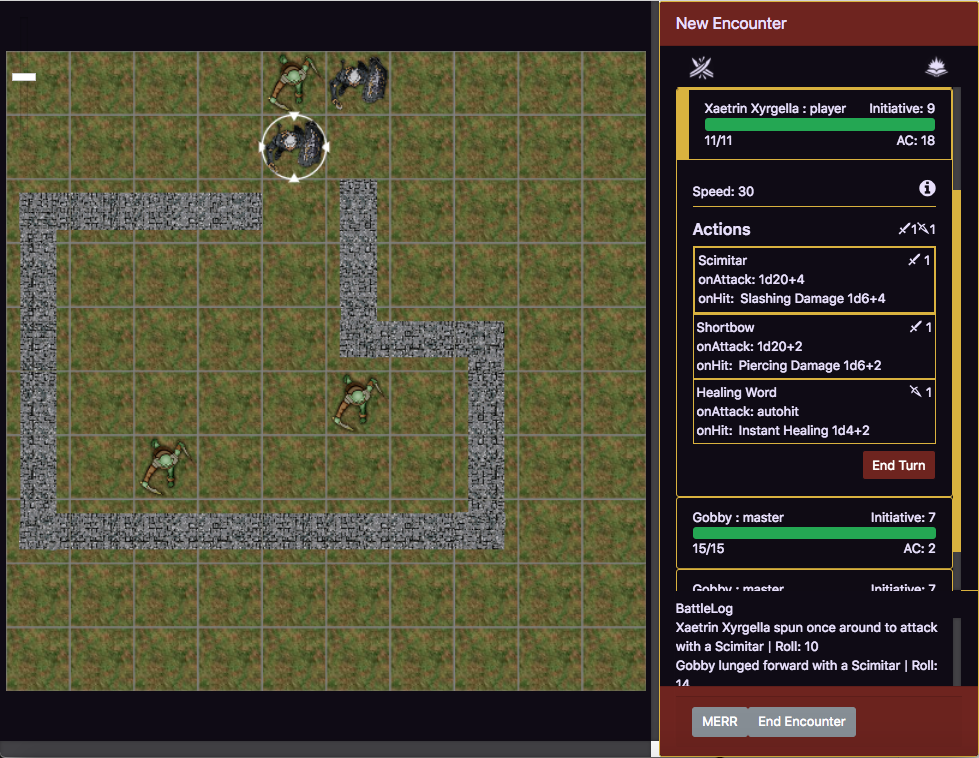
\includegraphics[scale=.5]{encountercreator}
	\caption{Battlefield Prototype}
	\label{fig: Battlefield Prototype}
\end{figure}
Above is a early prototype of our Battlefield. It contains three separate components: the main battle board, the sidebar, and the combat log. 
\subsection {The Battle Board }
The Battle Board is where all the environment, obstacles, and combatants are rendered. The board is a 2d top down arena, inspired by popular strategy games such as Civilization. The board is composed of checkerboard likes faces Each of which represent 5 feet of space in the game world. Obstacles and combatants will be rendered inside of these spaces. Obstacles and combatants can be hovered over and selected as well as click and drag into other spaces within the combatants movement range. If one of the combatants or obstacles are clicked their details and descriptions will appear in the sidebar. 
\begin{figure}[H]
	\centering
	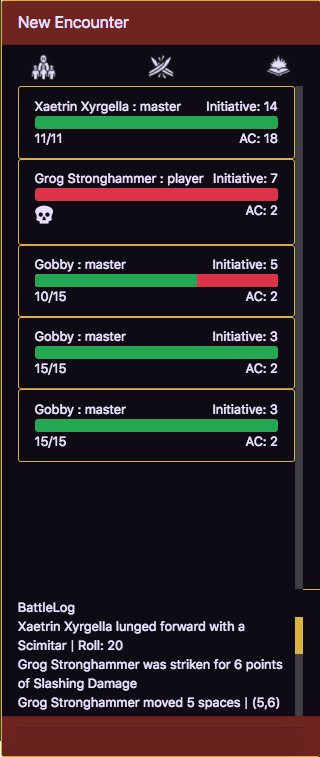
\includegraphics[scale=.5]{encountercreatorsidebar}
	\caption{Battlefield Prototype Sidebar}
	\label{fig: Battlefield Prototype Sidebar}
\end{figure}
\subsection {The Sidebar }
In the sidebar the user can view a combated or obstacles description and statistics. If the user selected a combatant the user will also be able to browse the combatants actions and on the combatants turned use those actions in combat. The sidebar is also where the user will control his combatant honest turn in combat whether it involves rolling initiative, performing actions, adjusting equipment and stats, or ending the turn itself. The sidebar will also be used in the creation mode of the battlefield. In the sidebar the user will be able to search, select, in drag combatants and obstacles onto the battlefield. They can also view and edit any of the stats using a form contained in the sidebar. The sidebar will also be where the user can make adjustments to combatant AI whether it's setting its aggressiveness level or selecting one of our built in my presets. In other words the sidebar is where the user will manage all the details of the encounter in both creation and playing modes. 
\subsection {The Battlelog }
The Battlelog below is where all of the messages attached to combat an encounter actions will be displayed. They will supply the user with an up-to-date text rendition of the encounter. It will include messages like, "The Goblin struck the cleric with a sword dealing 5 points of slashing damage", "The wizard casted Firebolt at the ogre but it missed", and "The Rogue hides behind the barrel the dragon does not seem to notice him". Early on in the Battlelog implementation we plan for very simple straightforward statistical messages that will aid us during testing and AI development. However we are planning to expand this feature to aid in role-play. We feel that having more colorful destruction of the actions occurring in the encounter. Will add another layer of fun for the user. 
\subsection {States and Controllers }
The same battle components will be used for both creation of the encounters and playing of the encounters. The controller will either hide or allow the user to view certain tools depending on what state the user has entered the battlefield in. For example if the user was in creation mode, they would also have access to our database of built-in combatants and obstacles said they will be able to add to their encounter. 
\subsection {Future Implementation/Design Plans }
Stated earlier this is a early prototype created in Angular 4 using Bootstrap for the UI. We plan on porting the system over to React and using fabricjs and HTML5 canvas to construct the Battle Board. This will give us a lot more freedom with red during the environment including varied combating in obstacle sizes and easier drag-and-drop capabilities. We also plan for the battlefield to take out the entirety of the players Street. The sidebar and the Battlelog themselves will be toggleable by clickable buttons on the sides and bottom of the screen. The battlefield will exist on its own component separate from the rest of the site so the overlaying UI such as the header and sidebar of the main site will not interfere with the battlefield experience.
	\newpage
	\section{Color Scheme}
	\begin{figure}[H]
		\centering
		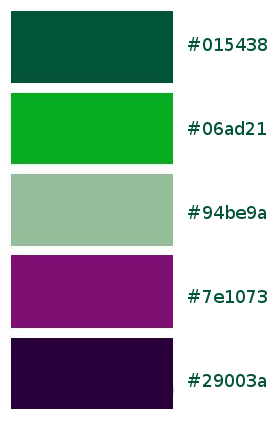
\includegraphics[scale=.5]{colors}
		\caption{Color Scheme}
		\label{fig: Color Scheme}
	\end{figure}
	When choosing a color palette to build our website, we looked around at other websites that focused on role-playing game topics and at gaming sites as well. The majority of these sites opt for a black and red or some combination black and X style when creating their look and feel. With Critical Encounters we wanted to break a little bit out of the norm and use colors that really pop out at the user, really make an impression on them, and set ourselves a bit apart from the other cites that they have been to.
	\newpage
	\section{Icons}
	Most of the icons we utilize will be provided by the free icon APIs font-awesome and rpg-awesome. Additional icons will be acquired through Game-Icons.net.
	\subsection{rpg-awesome}
	\begin{itemize}
		\item 
\includegraphics[scale=.06]{dashboard_icon}
		The Dashboard icon is used in the navbar and on the Dashboard itself to indicate where the user is on the site.
		\item 
\includegraphics[scale=.03]{arena_icon}
		The Arena icon (depicted as a house crest) represents the users' Arena and is used in the navbar and on the Arena page itself to indicate where the user is on the site.
		\item 
\includegraphics[scale=.03]{sword_lightning}
		The total number of plays in an Arena has the sword crossed with lightning icon. It appears on the users' Arena as well as on the Encounter Page itself.
		\item 
\includegraphics[scale=.03]{win_rate}
		The trophy pedestal icon represents the percentage of users that have defeated/finished the respective encounter.
		\item 
\includegraphics[scale=.03]{scroll}
		The unfurled scroll indicates how many reviews/comments have been given to an encounter.
		\item 
\includegraphics[scale=.07]{rating_icon}
		The star (intuitively) represents the rating that an encounter has received by users that have finished the given encounter. It is depicted on the Arena page, filtering of the search results page, as well as the Encounter Page.
		\item 
\includegraphics[scale=.03]{subscribers_icon}
		The subscribers icon falsely represents the physical appearance of all those that utilize Critical Encounters. It also represents the number of users that are subscribed to that Arena, and is present on the Arena page.
		\item 
\includegraphics[scale=.03]{plays_icon}
		The number of plays an encounter has had is shown in the Encounter Stats column on the encounter page, and is represented by the figure of two axes crossed. Game on.
		\item 
\includegraphics[scale=.03]{pc_deaths}
		The iconic skull \& crossbones icon indicates how many PC Deaths the encounter has accrued over its' lifetime. It is present on the Encounter Page.
		\item 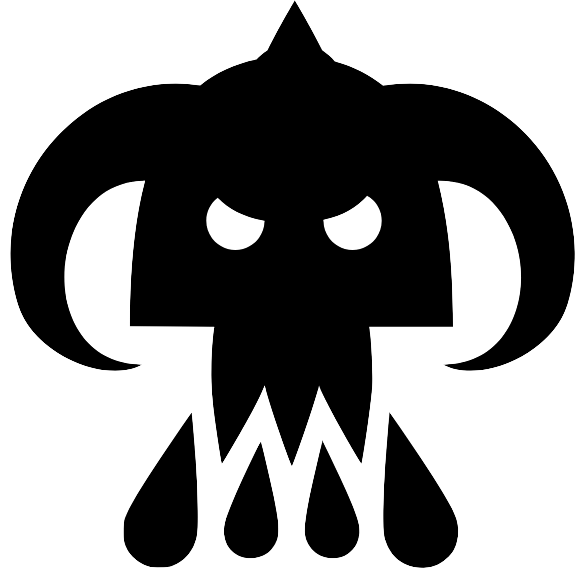
\includegraphics[scale=.03]{npc_deaths}
		A figure wearing an iron helm represents the number of NPC deaths that have occurred in an encounter. Whether this was due to the PCs' or their own infighting is left ambiguous. It is present on the Encounter Page.
		\item 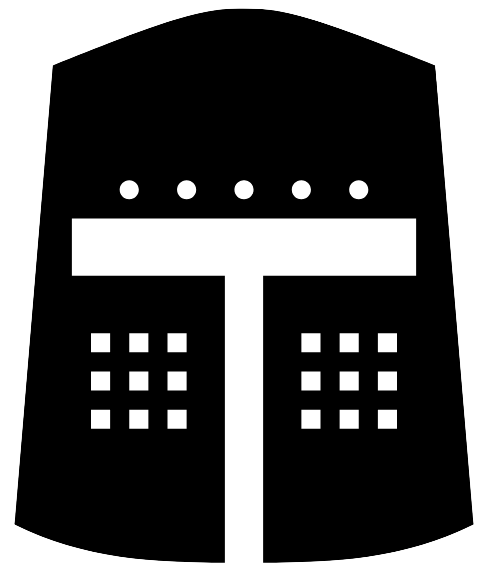
\includegraphics[scale=.03]{most_popular_class}
		This icon shows the class that was chosen most by users when playing through this encounter. It appears on the Encounter Page.
		\item 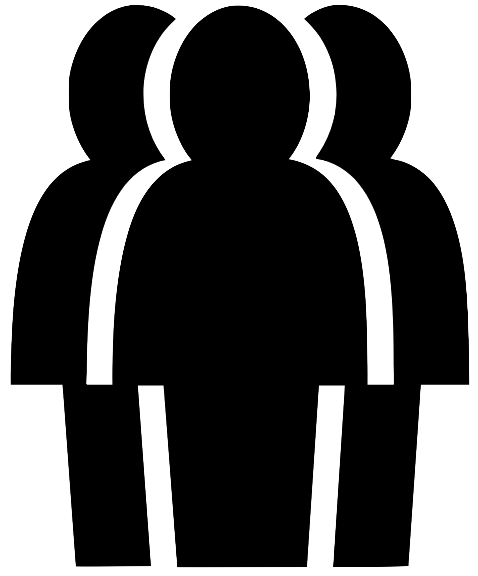
\includegraphics[scale=.03]{most_popular_race}
		Races in roleplaying games can drastically change the shape of a class, and tilt the advantage of an entire encounter with the right abilities in place. The race that was chosen the most in this encounter is represented by this icon.
		\item 
\includegraphics[scale=.03]{avg_rounds}
		The stopwatch indicates how long an encounter generally lasts, counted in the number of rounds that are played through in the combat. It is located on the Encounter Page.
	\end{itemize}
\newpage
	\subsection {Logo}
	\begin{figure}[H]
		\centering
		
\includegraphics[scale=.5]{logo-large}
		\caption{Critical Encounters' Logo}
		\label{fig: Critical Encounters' Logo}
	\end{figure}
	We wanted the logo design to accompany the overall UI design choices of the website with a more simplistic approach, while also representing the RPG aspect of Critical Encounters. We decided on a helmet because it gave a little more of a human feel, we thought swords or other weapons would be too inanimate and maybe even a bit cliché. Because of the light green color, and the contrast of our darker purple color choice with the navigation bar, this logo will "pop" on all of the views on the website(Figure \ref{fig: Critical Encoutners' Logo with Background}). The logo can also be easily scaled to fit most container sizes, which fits in to our application's versatility between desktop and mobile browsers.
	\bigskip
	\begin{figure}[H]
		\centering
		
\includegraphics[scale=1]{navbar-logo}
		\caption{Critical Encounters' Logo with Background}
		\label{fig: Critical Encounters' Logo with Background}
	\end{figure}
\newpage
\chapter*{Technical Goals}
This project is designed to streamline the process of creating a role-playing game's encounter, while also providing new advantages to further improve the encounter's quality. By handling the calculations computationally, as opposed to by hand, along with the ability to test the encounters, GMs will be able to perfect their encounter in preparation for when the encounter is played live.

This project will be a hurdle for everyone on the team as we are diving into information that many of us only know a little about. While we are relatively new to web frameworks, databases, and AI, we are determined provide a fully functioning d20 encounter creation and sharing platform.
\stepcounter{chapter}
\addcontentsline{toc}{chapter}{Technical Goals}
	\section{Overall Goals}
	Critical Encounters is going to require many moving pieces working together to deliver the product we intended. The original goal of the project was to create a platform that allowed users to create, test, and share encounters with other users. In order to satisfy this goal, these pieces have been individually broken down below:
		\subsection{Encounter Creation}
		The creation of the encounter itself is one of the fundamental functions of Critical Encounter. The Encounter Creator is going to be an easy to use platform that users can create encounters by drag and dropping entities onto an interactive virtual board that acts as the role-playing game's encounter arena. This will also require the ability to have specific variables relating to player characters, enemy characters, and obstacle objects. The ability to alter enemy statistics and behavior are also necessary.
		\subsection{Battle \& Stress-test}
		Once an encounter is created, the user has the ability to play through the encounter as the player character while Critical Encounter controls the enemy AI. The encounter will follow the standard d20 rule set to provide as realistic of an encounter experience as possible, in order to give the GM a good idea of how the encounter plays out (not to mention that it's fun).
		
		Along with this, the Stress-tester is a function that allows the GM to run their encounter numerous times with changes in various qualities of the player's party. The stress tester will run several times for each different iteration and display statistics of the overall battles at the end of the test. These statistics will include win/loss ratio, average battle length, number of player deaths/kills, as well as bring note to any outlier situations that may have proved the encounter or the players are overpowered.  
		\subsection{Enemy AI}
		It is necessary for Critical Encounters to have a properly functioning AI in the battles and stress-tests. In order to simulate the actual encounter experience, the enemies need to make their decisions independently, so that the player character can actually battle against something. The AI doesn't require intense machine learning, but will need a basic Attack/Defense strategy. The AI will assess the situation through a series of checklists in order to make the best move possible against the player. Along with this, AI behavior will need to be able to be altered leaving the enemy more/less aggressive, focus more on support than attack, etc.
		\subsection{Encounter Sharing}
		Once an encounter is created, the GM will be able to upload their creation to their Arena. This will act as a user profile displaying all of their created encounters/players/enemies. Other users can look at other's profiles and play through their encounters. Encounters will require a rating system that will follow a 5 star format, along with an optional written review.
		
		Encounter sharing will require a working search bar that will allow you to find specific encounters. There will be a search criteria that will include encounter name, type of encounter, party size, level range, etc.
	\section{Project Timelines}
	Our project takes place over two full semesters as part of the courses Senior Design I and Senior Design II. There are two major milestones that correspond to the end of each semester. The primary deliverable for semester one will be the final design document. Although the final design document will be the primary focus of semester one, we will also be focused on making small but meaningful progress in our implementation in order to have a solid head start for the second semester. The final deliverable for semester two will be the completed system as described in the design document. 
	
	There will be a period of time between the two semesters in which no milestones are listed. However, this time will be used to make small foundational progress towards the implementation of the final system in order allow for the smoothest transition into the implementation phase as possible. 
	
	Each semester will be broken down into a smaller organized list of milestones. Each of these milestones will have a deadline which should be met. The list of these milestones is show in Table \ref{table: milestones}
	
	\begin{table}[H]
		\begin{center}
			\begin{tabular}{ |c|c| } 
				\hline
				Milestone: & Completion Date: \\
				\hline
				Define Requirements/Initial Project Proposal & 10/9/2017 \\
				Verify Requirements & 10/16/2017 \\
				Decide Development Model & 10/23/2017 \\
				Define Sections & 10/30/2017 \\
				First Project Presentation Draft & 11/13/2017 \\
				Assign Design Document Sections & 11/20/2017 \\
				Senior Design Final Document & 11/29/2017 \\
				Web App Board And Gameplay & 1/9/2018 \\
				AI Prototype For DM and PC & 1/18/2018 \\ 
				PC Save/Load & 1/25/2018 \\
				Encounter Save/Load & 2/1/2018 \\
				Save/Load To Server & 2/12/2018 \\
				Browser Search And Play & 2/28/2018 \\
				Browser Ratings/Follows & 3/5/2018 \\
				Encounter Tester Implementation & 3/12/2018 \\
				Encounter Tester Statistics/Feedback & 3/19/2018 \\
				Advanced AI (Additional Settings, Counters) & 3/30/2018 \\
				Encounter Tester Advanced Features & 4/9/2018 \\	
				\hline
			\end{tabular}
		\end{center}
		\caption{Milestones} \label{table: milestones}
	\end{table}
	
	\section{Communication}
	\begin{wrapfigure}{r}{0\textwidth}
		
\includegraphics[scale=.15]{slack}
		\caption{Slack}
		\label{fig: Slack}
	\end{wrapfigure}
	Before our actual first meeting as a team, and as soon as we knew our team composition, we immediately set up a Slack group specifically for quick and constant communication to be available. We are using and will continue to use Slack as a means to keep up with each others' progress on individual goals, as well as keeping ourselves available to questions pertaining to those individual goals that other members might have during development. Slack also allows for easy file transfer, group check-ins, task/milestone reminders, notifications (specifically on commits and pushes to our GitHub repository), and discussions for the project. \par
	\begin{wrapfigure}{l}{0\textwidth}
		
\includegraphics[scale=.06]{trello}
		\caption{Trello}
		\label{fig: Trello}
	\end{wrapfigure}
	We are also utilizing another means of communication that specializes in the realm of project management: Trello. Using Trello has allowed us to break apart this semester's documentation task and therefore given each of us the ability to focus on our own sections without the need to wait for each others' work to continue our own. By assigning tasks on the Trello board, we have split ourselves into teams that focus on different areas of this document. So, when there are questions pertaining to that specific area, we have another member of the team also assigned to that task that we can turn to. Trello has allowed us to plot out the time that we need for each section very well, and therefore we will continue to use Trello next semester for production of our web application.
	\section{Research}
	Research for the tools we will utilize going forward with Critical Encounters was performed by the members of the team that will be the most involved with those tools. This approach is pretty intuitive, but also allows for those members who perhaps do not have much experience in the realm of website development or algorithm creation a chance to gain a base for which to stand on during the development stage. Once our members have researched the tools, at the very least we will be able to start from there and build up.
	\section{Budget}
	With this project, we are going to be utilizing the fact that this program will be for personal use to avoid nearly all costs to us. For the time being, we are using completely free to use platforms as well as not infringing on any copyrights or patents, by doing things like opting for using the D20 Game System as a base for our ruleset (which is free to use without conflict), instead of utilizing a similar but copyrighted and highly policed set of rules like D\&D's 5th Edition ruleset. For us to build the program and run them on local machines should cost us no more than valuable time and electricity bills. When the program nears completion we will be assessing the option of pushing the program to a server which is where money would start to be involved.
	
\newpage
\chapter*{Application Design}
\stepcounter{chapter}
\addcontentsline{toc}{chapter}{Application Design}
	\section {High Level Design}
		\begin{figure}[H]
			\centering
			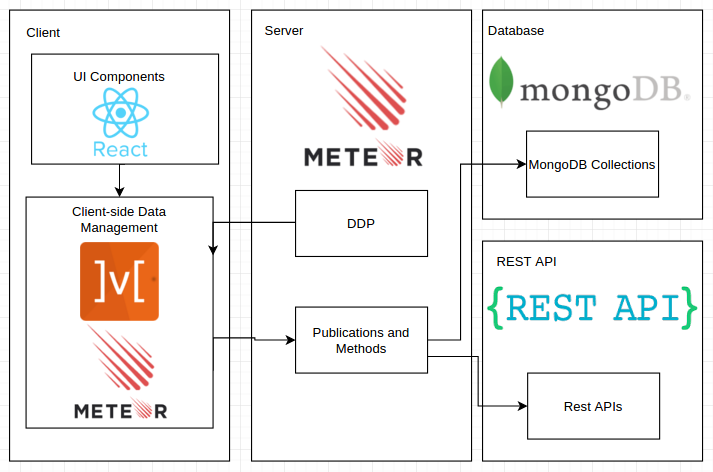
\includegraphics[scale=.5]{designsd.png}
			\caption{High Level Design Diagram}
			\label{fig: High Level Design}
		\end{figure}
		
		\paragraph{}We will be implementing a Client-Server Design structure that is commonly used with web apps such as Critical Encounters. There are three areas of production in this high-level design: Server, Database/Rest API and Client-Side. The UI components will be developed in REACT and will control the the MVC system. Data management on the client-side will be managed by MobX and Meteor, the latter of which will server as the point of contact with the server-side of the app. The server will also be developed in Meteor, and will be responsible for contacting the database, developed in MongoDB and performing REST API commands when necessary. \par
		 The relationship between client and server will be a sudo model-view-controller architecture. Where REACT will act as the as application's view and Meteor/MobX will act as both the controller and the model. Meteor with MobX will automatically manage the data flow, client state, and client rendering.
	
	\section {Design Patterns}
		
		\begin{figure}[H]
			\centering
			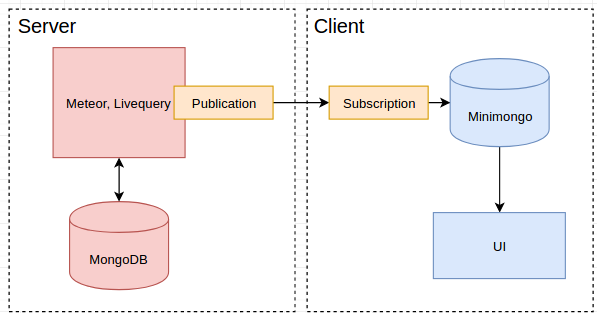
\includegraphics[scale=.7]{orm.png}
			\caption{Design Pattern Figure}
			\label{fig: Design Pattern Figure}
		\end{figure}
		
		\paragraph{} Meteor uses implements a ORM/MERN, Object-relational mapping / MongoDB - Express - React, stack design pattern. It focuses on model driven development, in which the models are shared between the server and the client. This is seen most clearly seen in the MiniMongo database cache that is accessible by the font-end front end and can asynchronously update the MongoDb REST API is implemented automatically which translates to automatic database updates.

\newpage
\section {Server Design}
	\subsection{Meteor}
		\begin{wrapfigure}{l}{0\textwidth}
			
\includegraphics[scale=.2]{meteorJS}
			\caption{Meteor.js}
			\label{fig: Meteor.js}
		\end{wrapfigure}
		Meteor is a full-stack JavaScript platform for developing modern web and mobile applications. Meteor includes a key set of technologies for building connected-client reactive applications, a build tool, and a curated set of packages from the Node.js and general JavaScript community.
		
		
		
		On the client, there is no direct connection to the MongoDB database, and in fact a synchronous API to it is not possible (nor probably what you want). Instead, on the client, a collection is a client side cache of the database. This is achieved thanks to the MiniMongo library—an in-memory, all JS, implementation of the MongoDB API. What this means is that on the client, when you write:
		
		\begin{lstlisting}
			const Users = new Mongo.Collection('users');
		\end{lstlisting}
		
		It creates a new collection in the MongoDB database called 'users' and assigns the collection to the variable Users. Now you can send queries and updates to the database:
		
		\begin{lstlisting}
			// Return an array of useres with name Hunter
			const allUsers = Users.find({ name: 'Hunter' }).fetch();
			
			// Create a new user.
			Messages.insert({ name: 'hunter', email: 'hunter@gmail.com', validated: false });
			
			// Validate user
			Users.update(allUsers[0]._id, { $set: { validated: true } });
		\end{lstlisting}
		
		
		
		
		\begin{tabular}{ |p{3cm}||p{3cm}|p{3cm}|p{3cm}|  }
			\hline
			\multicolumn{4}{|c|}{Meteor Database} \\
			\hline
			Country Name     or Area Name& ISO ALPHA 2 Code &ISO ALPHA 3 Code&ISO numeric Code\\
			\hline
			Afghanistan   & AF    &AFG&   004\\
			Aland Islands&   AX  & ALA   &248\\
			Albania &AL & ALB&  008\\
			Algeria    &DZ & DZA&  012\\
			American Samoa&   AS  & ASM&016\\
			Andorra& AD  & AND   &020\\
			Angola& AO  & AGO&024\\
			\hline
		\end{tabular}
		
	\subsection{Server Sequence Diagrams}
	\subsubsection {Encounter Search SSD}
		\begin{figure}[H]
			\centering
			\centerline{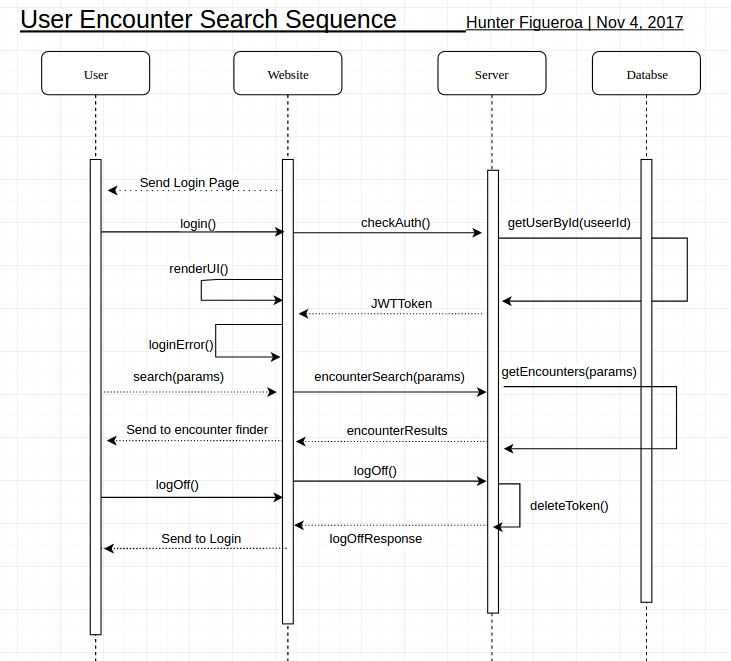
\includegraphics[scale=.7, angle=90]{ssd_encounter_search}}
			\caption{Encounter Search SSD}
			\label{fig: Encounter Search SSD }
		\end{figure}
	\newpage
	\subsubsection {Encounter Feed SSD}
		\begin{figure}[H]
			\centering
			\centerline{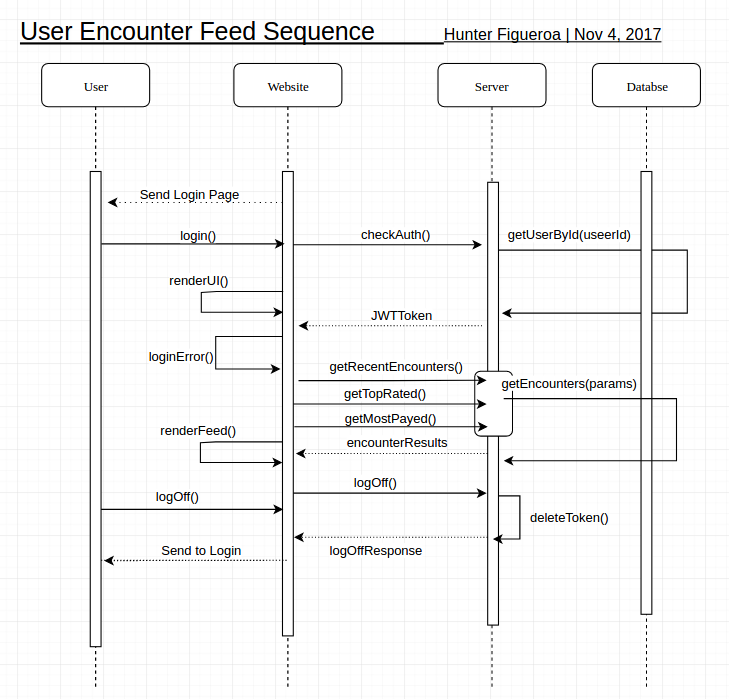
\includegraphics[scale=.7, angle=90]{ssd_encounter_feed}}
			\caption{Encounter Feed SSD}
			\label{fig: Encountner Feed SSD }
		\end{figure}
	\newpage
	\subsubsection {Arena Subscription SSD}
	\begin{figure}[H]
		\centering
		\centerline{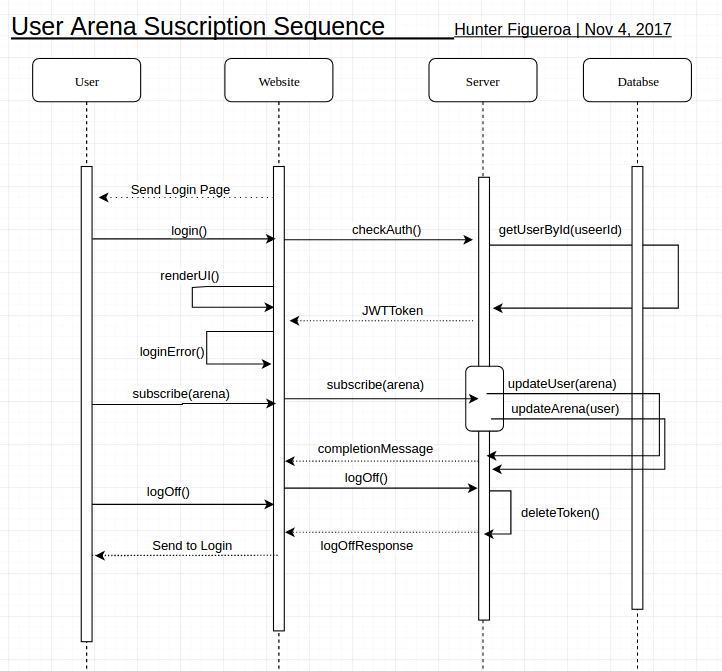
\includegraphics[scale=.7, angle=90]{ssd_subscribe}}
		\caption{Arena Subscription SSD}
		\label{fig: Arena Subscription SSD }
	\end{figure}
\newpage
\section{Database Design}
\subsection {Database Diagram}
\begin{figure}[H]
	\centering
	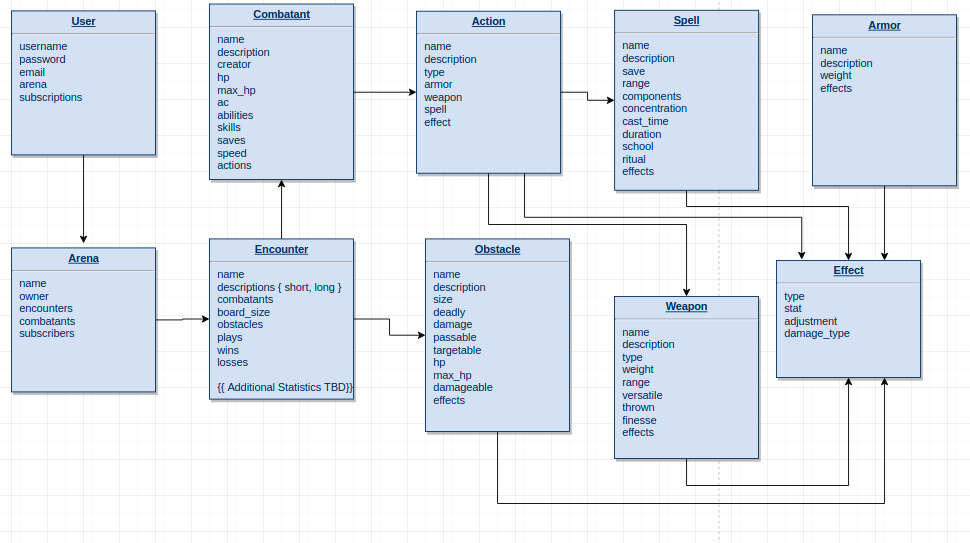
\includegraphics[scale=.4]{database_schema}
	\caption{Databse Schema}
	\label{fig: Databse Schema }
\end{figure}
\subsection{Schema}
Below are schema that will be used to structure the MongoDB collections. The schema themselves will be implemented in Meteor using their MongoDB schema syntax and design. Below is an example of the schema representation of a Critical Encounter user collection:

\begin{lstlisting}
Users.schema = new SimpleSchema({
username: {type: String, required: true},
password: {type: String, required: true},
arena: {type: String, regEx: SimpleSchema.RegEx.Id},
subscriptions: [{type: String, regEx: SimpleSchema.RegEx.Id}]
});
\end{lstlisting}

The general structure is a field name and a matching feild type (String, Boolean, Object ) with optional requirements or parameters (regEx: SimpleSchema.RegEx.Id).

Note: The { "Collection Name" } notation represents an Object.id that correlates to a MongoDB object of that collection type
\subsubsection{User Schema}
\begin{figure}[H]
	\centering
	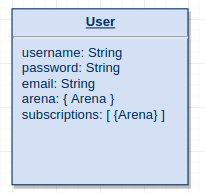
\includegraphics[scale=.75]{schema-user}
	\caption{User Schema}
	\label{fig: User Schema }
\end{figure}

\paragraph{}This schema will hold basic user information: identification information (username, password), a reference to their Area (Arena), and a list of the Arenas they are subscribed to (subscriptions). This is the entrance point for all data accessible on the website. All other collections on the database are associated with at least one user object and has only one user owner/creator. All login and authentication information and routing will referenc the user collection to confirm identification. The password string will be saved as a string that has been encrypted to protect user information.

\subsubsection{Arena Schema}

\begin{figure}[H]
	\centering
	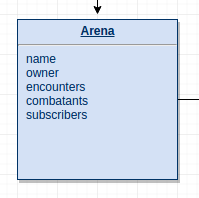
\includegraphics[scale=.75]{schema-arena}
	\caption{Arena Schema}
	\label{fig: Arena Schema }
\end{figure}

\paragraph{}This schema will hold basic Arena information: an Arena name (name), a reference to Arena's creator: (owner), a list of encounters that are contained in the arena (encounters), and a list of references to users that are subscribed to the (subscribers). The Arena acts as a hub, organizer and access or for every user and their encounters. Arena statistics are not directly maintained in the Area object itself but are compiled from the list of encounters that is contained in the encounters field. This allows the statistics as up to date as possible without constantly updating both area statistic and the encounter statistics when an encounter goes through a stat change.

\subsection{Encounter Schema}
\begin{figure}[H]
	\centering
	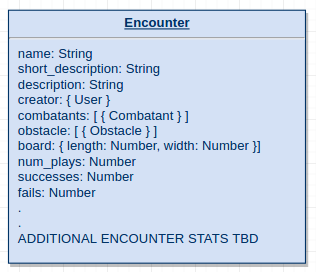
\includegraphics[scale=.75]{schema-encounter}
	\caption{Encounter Schema}
	\label{fig: Encounter Schema }
\end{figure}
Encounters created by a user will be saved in a encounter document using this schema. It will contain basic descriptive information: name, descriptions, creator. As well as physical details about the encounter itself: an array of obstacles, an array of combatants, board size. The encounter will also contain statistical information useful for both players and game masters: number of plays, success rate, most played class. This is  where statistical data is stored, these statistics will flow upward and be adjusted and displayed on other components such as arena statistics.
\subsection{Combatant Schema}
\begin{figure}[H]
	\centering
	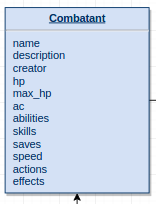
\includegraphics[scale=.9]{schema-combatant}
	\caption{Combatant Schema}
	\label{fig: Combatant Schema }
\end{figure}
This schema will be used to represent all combatants in an encounter, both player and non-player characters. All of the base stats for the combatant are stored in the document. All bonuses will be added after so it is easy to add and remove bonuses to combatant stats. Stat modifiers will also not be calculated using the respective modifier formula as well as adding additional bonuses from any effects the combatant has received from items, features and abilities. We designed the the schema this way to keep the database uncomplicated so it will be easier to edit and create new combatants. The combatant document will also contain a array of actions that the combatant can take on its turn. These actions will be displayed and selectable in the Battlefield sidebar on the combatants turn and combat.  All combatants will be assigned a reference to its creator. Most of the combatants at first implementation will be under Critical Encounters' user ID and they will be available to use for all users. This feature will also make it easy to implement creature and combatant sharing sometime in development or as a stretch goal.
\subsection{Obstacle Schema}
\begin{figure}[H]
	\centering
	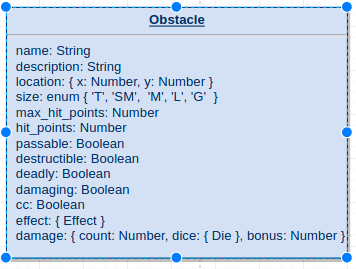
\includegraphics[scale=.9]{schema-obstacle}
	\caption{Obstacle Schema}
	\label{fig: Obstacle Schema }
\end{figure}
This schema contains data for non-combatant entities in an encounter, i.e. entities that do not have a turn in combat and do not roll initiative. Examples of obstacles are walls, traps, doors, inanimate objects, water, holes, and items. The schema outlines basic descriptive information information name, description and size, as well as a range of boolean values that describe the obstacle's role and interaction with players in combat. For example, a bottomless pit would have the deadly boolean set to true so any combatant that were to fall in it would die instantly. Walls on the other hand would have the passable boolean set to false, which will stop the AI pathfinder from choosing a path through walls. The obstacle will also have an array of Effects. These  effects would include any Crowd Control, Damage, Healing or Magical effects the obstacle might have. This includes damage for traps, half speed for traveling through brush, and magical healing aura from enchanted statures. The implementation of the effects may change to bettersuit the implementation of the AI combat and encounter flow.
\subsection {Action Schema}
\begin{figure}[H]
	\centering
	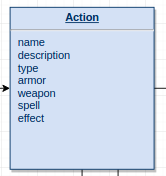
\includegraphics[scale=.9]{schema-action}
	\caption{Action Schema}
	\label{fig: Action Schema }
\end{figure}
The action schema contains data about actions combatants will be able to take on their turn. The actions stored in the database will be restricted to actions given gained from items, features, classes, and races. Actions available to all combatants, movement, disengage and dash for example will be hard coded for all combatants to avoid bloating the database. The purpose of an action document is to describe the action and its requirements. Little computational work will be done directly to the action document, instead it will be done with the action's effects.
\subsection {Effect Schema}
\begin{figure}[H]
	\centering
	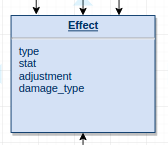
\includegraphics[scale=.9]{schema-effect}
	\caption{Effect Schema}
	\label{fig: Effect Schema }
\end{figure}
The effect schema will be were most of the computational data will be held. It will be held as reference by many other documents such as armor, weapons, and features. Effects adjust player stats like health, strength, and speed. They can apply a flat bonus or reduction, half, double or triple statistics, or apply a advantage or disadvantage to stat checks. The stat change will be described in the type
\subsection {Spell Schema}
\begin{figure}[H]
	\centering
	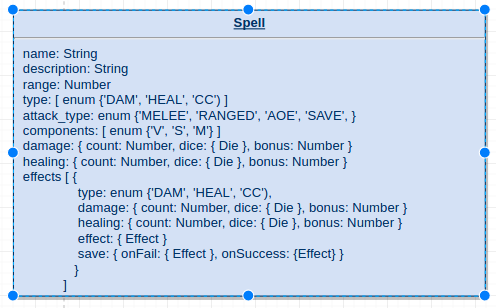
\includegraphics[scale=.9]{schema-spell}
	\caption{Spell Schema}
	\label{fig: Spell Schema }
\end{figure}
This schema describes a spell associated with a combatant action in game it contains description information as well as an array of the spells effects describes inside effect objects.We decided to construct a spell very modularly and easily customizable so that sometime in future development we can easily implement a to allow users to create and edit their own spells.Most of what the AI is going to interact with in a spell document is with the array of Effect objects.
\subsection {Weapon Schema}
\begin{figure}[H]
	\centering
	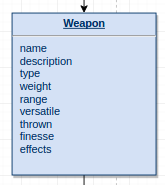
\includegraphics[scale=.9]{schema-weapon}
	\caption{Weapon Schema}
	\label{fig: Weapon Schema }
\end{figure}
This schema describes a weapon that can be equipped by a combatant. Weapons are referenced in actions and the data the weapon contains, their flat stats such as damage and range and their referenced effects. These effects are implemented by the AI the actions during combat.

\subsection {Armor Schema}
\begin{figure}[H]
	\centering
	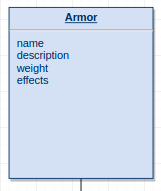
\includegraphics[scale=.9]{schema-armor}
	\caption{Armor Schema}
	\label{fig: Armor Schema }
\end{figure}
This schema describes an armor that can be equipped by a combatant. Armor is referenced in actions and the data the armor contains, their flat stats such as armor class and weight and their referenced effects. These effects are implemented by the AI the actions during combat.
\newpage
\section{Client Side Design}

	\subsection{URL and Routing}
		There are two options to font-end routing for using our stack: React-Router and Meteor's FlowRouter. Both implementations have their pros and cons but after some research and deliberation we have decided to use Meteor's FlowRouter. The notation and syntax for FlowRouter is much more clear and easier to learn. There haws also been a history of React-Router not playing too well with Meteor applications. 
		
		FlowRouter is relatively straight fore-ward and is composed of two main components, the URL and the action. In short when the URL is accessed by the browser the action is triggered. In our case the action method will most likely be a ReactLayout render call to render react components associated with that route to the view.
		
		Below is a routing example for the dashboard page of Critical Encounters:
		
		\begin{lstlisting}
			FlowRouter.route( '/dashboard', {
				name: 'dashboard',
				action() {
							ReactLayout.render( App, { yield: <DashBoard /> } );
				}
			});
		\end{lstlisting}
		
		\subsubsection { URL Routes}
		
			\begin{table}[H]
				\begin{center}
					\begin{tabular}{ |p{5cm}|p{7cm}|| } 
						\hline
						URL Route: & Purpose: \\
						\hline
						/dashboard & Routes users to dashboard page \\
						/account & Routes current user account information\\
						/encounter-finder/:query & Route to search result page accessible at anytime through the fixed header search bar  \\
						/arenas/:arenaName & Route to area with specified arena name  \\
						/encounters/:id & Route to encounter with specified id \\
						/battlefield/creator/:id & Enter Battlefield in creator mode with given encounter id \\
						/battlefield/player/:id & Enter Battlefield in player mode with given encounter id \\
						/battlefield/master/:id & Enter Battlefield in master mode with given encounter id \\	
						\hline
					\end{tabular}
				\end{center}
			\caption{URL Routes} \label{table: URL Routes}
		\end{table}
		
	\subsection{Types of Views and Controllers}
	While React does not use a Model-View-Controller architecture for development, it does have things such as ``View Controllers" and ``Controller Views" that are top level components which hold all states, and passes those to child components as props. \cite{reactcvp}
		\subsubsection{AccountController}
		\subsubsection{DashboardController}
		\subsubsection{ArenaController}
		\subsubsection{EncounterPageController}
		\subsubsection{EncounterBrowserController}
		\subsubsection{BattlefieldController}
	
	\subsection{Battlefield Modes}
		\subsubsection{Game Mode}
			This is the main mode available in the Critical Encounters Battlefield. In this mode users will be able to play, simulate, and view and gather data about their own encounters as well as other user's.
			\subsubsection{Role: Player}
				Player is in control of a single player character and can either control his character directly in combat or apply an AI to his player character. every round the player will perform his/her character's actions on its turn. Once complete the AI will simulate all other combatant's turns and refresh the battlefield. Once the encounter is complete the player will be able to view his character's stats and results from the encounter.
			\subsubsection{Role: Game Master}
				Controls multiple combatants against a one or more player characters. The game master on each turn can choose to either simulate the combatant's turn or perform the actions on the combatant's turn manually using the AI. After the encounter has completed there the game master will be able to review the encounter stats and results.
				
		\subsubsection{Creation Mode}
			\subsubsection{Role: Creator}
				There is only one role available for the Creation Mode: the Creator role. In this mode the user will be able to design their own encounters using the Encounter Creator Tools. Users will be able to add obstacles and combatants, as well as customize the combatants stats and AI presets. Once the user has completed creating the encounter the user may either publish the encounter, and perform Encounter Validation process or keep the encounter private for personal or invite use.
	\newpage
	\subsection{Map / Environments}
	\begin{figure}[H]
		\centering
		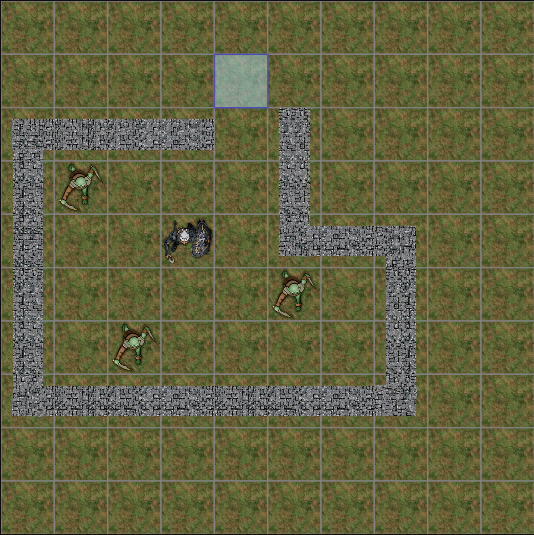
\includegraphics[scale=.6]{environment}
		\caption{Board with Obstacles}
		\label{fig: Board with Obstacles}
	\end{figure}
	In Critical Encounters, the map/grid that is usually utilized in tabletop gaming sessions for combat is transitioned into a virtual board with the same format. A grid where each square represents 5x5 spaces, images to represent characters and enemies, as well as obstacles. All of this is put in place to give the user familiarity with the encounter during their own testing, so that same familiarity is present when the encounter occurs with their own group. There will be a few maps that are developer-generated, to be used as a template for beginners to utilize, or for more advanced creators to build off of to build an even larger encounter. However, most of encounter creation will likely involve a creator generating their own map out of the provided components that Critical Encounters has to offer. For this reason, we will have a section of the database dedicated to storing as many viable choices for various characters, enemies, obstacles, and environment backgrounds that we deem useful.
	
	\newpage
	\subsection{Turn Structure / Order}
	Combat using the d20 System is composed of rounds in which each combatant in the encounter has one turn.  A round lasts 6 seconds in game time, during which all combatants act on their respective turns. Where a combatant's turn resides chronologically in a round is determined by the combatant's initiative roll (a combination of a dice roll and applicative bonuses). A turn it self is composed of 6 parts: Action(s), Bonus Action, Movement, Free Action, and Bonus Action, Reaction.
	\begin{itemize}
		\item Action
			\begin{itemize}
				\item The main action of a turn, every combatant has one or more per turn
				\item Ex. Attack, Cast a Spell, Dash, Disengage, Hide
			\end{itemize}
		\item Bonus Action
			\begin{itemize}
				\item An action gained by a feature, spell, or other abilities
				\item Ex: The Cunning Action feature allows a rogue to take a Bonus Action to hide, dash, or disengage
				\item Max one Bonus Action per turn
			\end{itemize}
		\item Movement
			\begin{itemize}
				\item Combatant can move the number of spaces equal to its speed (with applicaple bonuses) divided by five
				\item Some combatants also have swim and flight speeds that they can use as their movement action
				\item Multiple environmental restraints on this: Difficult terrain, attacks of opportunity
			\end{itemize}
		\item Free Action
			\begin{itemize}
				\item Interact with one object or environment 
				\item Ex: Open a door, you could draw your weapon
				\item interaction with more than one action requires the use of an action
			\end{itemize}
		\item Reaction
			\begin{itemize}
				\item Combatant has one of reaction in every round of combat
				\item Can happen anytime during the round, doesn't have to be combatant's turn
				\item Ex. Cast reaction spell, attack of opportunity
			\end{itemize}
	\end{itemize}

\section {Testing}

	For our testing we will be using a combination of both manual and automated testing. Automated testing will be performed using ReactTestUtils which will allow us to rapidly test front-end components. There is also a Meteor test tool that can be used to test both the client and servers sides of the application.

	Most of our efforts when it comes to testing our application will center around testing the AI. Since the AI is the most complex and most important part of the application we are doing to test it extensively so that users are satisfied with the primary feature of our application. To this end, we are focusing our efforts on developing the Battlefield as it will serve as a very useful tool to view and test output from the AI. Below is the order in which  we plan to test the AI. 
	
	\begin{itemize}
		\item Movement
		\begin{itemize}
			\item Combatant movement to target
			\item Combatant movement to target around obstacles
			\item Combatant movement when target is unreachable
		\end{itemize}
		\item Attacks
		\begin{itemize}
			\item Combatant melee attack when target is within melee range
			\item Combatant ranged attack when has line of sight and is within range.
			\item Combatant melee attack when target is not in range but is in movement range
			\item Combatant ranged attack when target is not in range but is in movement range
		\end{itemize}
		\item Spells
			\begin{itemize}
				\item Melee spell
				\item Ranged single target spell
				\item Ranged AOE spell
				\item Ranged line spell
				\item Ranged cone spell
				\item Spell Type Priority
				\begin{itemize}
					\item Damage
					\item Healing
					\item Crowd Control
				\end{itemize}
			\end{itemize}
		\item Alternative actions
		\begin{itemize}
			\item Dash to better position or out of attack range
			\item Disengage when threat is too great
			\item Hide when high treat or better position
		\end{itemize}
	\end{itemize}

Our plan for testing involving all components, both the search and profile layouts and the Battlefield, are summarized by the outline below:

\begin{itemize}
	\item{UI}
		\begin{itemize}
			\item Ensure that UI fits most desktop sizes 
			\item Ensure that the search bar is fixed in the header on all pages
			\item Ensure that the encounter feed output links to the correct encounters under the correct category
			\item Ensure that the search bar always redirects to the search page
			\item Display all correct stat data in arena correctly
			\item Ensure all buttons are cursor responsive and perform their correct actions
			\item Ensure that reviews are posted immediately under encounters
		\end{itemize}
	\item Data
		\begin{itemize}
			\item Ensure that correct encounter data is gathered, parsed and available for use in the Arena page.
			\item Ensure that new data from encounters is processed correctly and updated in the arena and encounter statistics
			\item Ensure that correct data is loaded to the Battlefield sidebar for use in both creation and play modes
			\item Ensure all encounter lists are correct in the dashboard page
		\end{itemize}
\end{itemize}
\newpage
\section{D20 Terminology}
		The D20 game system has variations from game to game whether it be changes to name, function, or practicality. Despite this, generally many the main qualities that the game styles have don't tend to stray too far from one another. While on this project, it is crucial that Critical Encounters should provide a broad enough experience to appease the largest portion of D20 games as possible so that players can apply their encounters to whatever D20 system they'd like. 
		\subsection{Character Terms}
			Within a character in the D20 system, there are many statistics, qualities, and abilities that help to determine how the character acts within the D20 world. These can alter attacks, defenses, skills, and even behavior.
		\subsubsection{Attributes}
			Attributes refer to the natural born characteristics that all characters within the game possess. Upon character creation, you choose to distribute a designated amount of points among several different attributes to create a truly unique character from the start. 
			Common attributes within the D20 systems are:
		\begin{itemize}
			\item Strength
			\begin{itemize}
				\item The character's innate physical capability. This can include the character's ability to carry items, melee damage, and preform physically demanding tasks (moving large items, barricading, holding enemies, etc.)
			\end{itemize}
			\item Constitution
			\begin{itemize}
				\item The character's health or stamina. Constitution determines the character's HP and endurance, as well as resistance to special damages. 
			\end{itemize}
			\item Defense
			\begin{itemize}
				\item The character's ability to resist damage. This is very similar to Constitution but ultimately different. This usually deals with direct hits from enemies and the character's resistance to HP deduction.
			\end{itemize}
			\item Dexterity
			\begin{itemize}
				\item The character's agility and hand-eye coordination. Dexterity allows the character to react quickly to attacks from enemies via dodging and counters. It can also effect the damage dealt to enemies, depending on the weapon. Certain weapons require more precision than strength alone, for example a battle-axe versus bow and arrow.
			\end{itemize}
			\item Intelligence
			\begin{itemize}
				\item This may be hard to guess, but Intelligence refers to how smart the character is. This can affect the character's ability to solve problems or understand foreign entities. For example, a character with high Intelligence may be able to decipher a clue via an Intelligence check.
			\end{itemize}
			\item Charisma
			\begin{itemize}
				\item The character's social ability. This mainly effects interactions between players and NPCs outside of an encounter. This can be used to barter prices and convince NPCs. Charisma can be used within an encounter through various ways such as intimidation. 
			\end{itemize}
			\item Wisdom
			\begin{itemize}
				\item The character's spirituality and common sense. Wisdom applies heavily in spellcasting and dealing with mystical qualities of the world. 
			\end{itemize}
			\item Perception
			\begin{itemize}
				\item The character's observation of their surroundings. Perception effects the character's chance towards noticing specific entities within the environment (hidden enemies, traps, clues, etc.)
			\end{itemize}
		\end{itemize}
		\newpage
		\subsubsection{Classes}
			Characters within the D20 are given roles to play throughout the campaign. Classes are chosen when the character is created and is fundamental in deciding how the character is going to play. The class affects the character's specific attributes in certain ways by adding extra points to some attributes and deducting points from others based on the class itself. Classes range from system to system but are all generally the same. The base classes are typically Barbarian, Rogue, Wizard, and Cleric, with many deviations of these classes within the individual D20 systems.
		\subsubsection{Alignment}
			\begin{wrapfigure}{r}{0\textwidth}
				\includegraphics[scale=0.25]{alignment}
				\caption{Alignment Table}
				\label{fig: Alignment Table}
			\end{wrapfigure}
			Every entity within the D20 system is given an alignment, Players and NPCs alike. This refers to the character's morals which is used for decision making. The alignment chart has two axis' that range from Lawful to Chaotic on one and Good to Evil on the other, with neutral in the middle of both of the axes. Typically enemy characters lie on the Evil spectrum but can be either Lawful evil to Chaotic Evil. Player Characters have no inclination to sway to the 'Good' spectrum of the table, although most players enjoy being the hero in a story and thus choosing that archetype. A PC could just as well be a heroic paladin as they could be a deceiving and conniving assassin.
		\subsubsection{Races}
			This refers to the character's actual species. Race (much like classes) give basic advantages and disadvantages to specific attributes, but also change provide minor changes to gameplay. Certain races will have certain abilities which can provide the party with advantages in battle. Races also vary from system to system but most follow a basic patter of human, elf, dwarf, half-orc, etc.
			
		\newpage
		\subsection{Combat Terms}
			There area variety of things that can occur during an encounter that effect the way the battle plays out. Certain terms appear every battle, while others only occur when specific occurrences line up. As these combat terms vary between systems, and some only occur in rare instances, a general list has been created to be used by Critical Encounters. Below is a compilation of terms that will most likely be utilized within an encounter, thought the terms used in the encounter may not be limited to this list.
		\subsubsection{Initiative}
			At the beginning of an encounter the player characters, NPCs, and enemies all roll for an initiative check. A D20 die is rolled and combined with the combatant's Dexterity modifier to establish the order that the combatant's perform their actions. The highest initiative roll goes first and it counts down from there.
		\subsubsection{Critical}
			When rolling for attacks, if the D20 die is rolled and lands on a 20, the highest number on the die, the attack lands as perfectly as it could. Provided that the attack beats the enemy's armor class, the attack deals the maximum amount of damage. Critical rolls are not limited to just attacks though, if a character is performing an action and gets a 20 the action is performed without flaw.
		\subsubsection{Botch}
			When rolling, the opposite of a critical can occur which is when the die lands on 1. This is a critical failure, which usually results in the character hurting themselves while failing the desired action.
		\subsubsection{Hit Points}
			Hit points (or HP) refers to the character's remaining health. If HP reaches 0, the character is rendered unconsious and is required to roll to prevent death. HP is lowered by receiving damage and replenished by potions, spells, or resting outside of battle.
		\subsubsection{Armor Class}
			This refers to the character's protective equipment and how well those items deflect damage. The stronger armor the character is wearing, the higher their AC is. If an attack is placed on someone and the damage the attack deals is less than the AC, the damage that would be dealt by the attack never occurs. 
		\subsubsection{Saving Throw}
			When certain threats occur such as traps being triggered or being poisoned, the receiving character must roll for a saving throw which could allow them to avoid the damage entirely.
		\subsubsection{Damage Types}
			Different attacks deal damage in different ways. Each damage type has pros and cons of being used in situations so players typically choose their attacks strategically in order to get the biggest advantage in an encounter. The damage types in  a standard d20 game are as follows. 
		\begin{itemize}
			\item \textbf{Bludgeoning} - Blunt force attacks. Can be dealt by enemies with hammers, clubs, or fists. Also includes falling and crushing damage.
			\item \textbf{Piercing} - Puncturing and impaling attacks. These can include weapons like spears or bites from monsters.
			\item \textbf{Slashing} - Standard damage done by swords, axes, claws, etc.
			\item \textbf{Poison} - Small amounts of damage over time. Dealt by venomous enemies, traps, or gas.
			\item \textbf{Magic} - There are a variety of spells within the D20 system which all deliver very specific types of damage. A few types are as follows:
			\begin{itemize}
				\item Fire
				\item Cold
				\item Force
				\item Lighting
				\item Psychic
			\end{itemize}
		\end{itemize}
		\subsubsection{Player Condition}
			There are a variety of states that character's can be in that alter their ability to perform certain tasks. These conditions can be altered by spells, class abilities, receiving an attack, etc. Conditions last a designated time depending on the method of delivery. Here is a list of possible conditions:
		\begin{itemize}
			\item \textbf{Blinded} - Combatant cannot see surroundings and fails perceptions checks. Combatant is given a large disadvantage.
			\item \textbf{Charmed} - Combatant cannot attack the charmer and is susceptible to social check by the charmer.
			\item \textbf{Frightened} - Combatant cannot willingly move closer to the source of fear. Combatant has a disadvantage on Ability and Attack rolls.
			\item \textbf{Grappled} - Combatant cannot move.
			\item \textbf{Unconscious} - Combatant cannot move, speak, or react to surroundings. Automatically fails saving throws. Combatant has disadvantage on all rolls.
			\item \textbf{Exhaustion} - Combatant is physically tired. Exhaustion works in several layers of intensity which range from having slower movement speed and disadvantage on abilities to the highest level, which is death.
		\end{itemize}
		\newpage
		\subsection{Modifiers}
			There are various qualities that could boost or deduct points for a character during an action. These qualities can be obtained from high stats, character class/race, or buffs from potions.
		\subsubsection{Attribute Modifiers}
			\begin{wrapfigure}{r}{0\textwidth}
				\includegraphics[scale=0.3]{modifier}
				\caption{Attribute Modifiers}
				\label{fig: Attribute Modifiers}
			\end{wrapfigure}
			Along with base values for all of the stats associated with a character are attribute modifiers. For each attribute, their score can range from 0-30. It is understood that an attribute score of 10 is a base score, any score lower than that results in a negative score modifier and any score higher results in a positive score modifier. Modifiers add or subtract for every 2 levels given. An ability score of 1 renders a -5 modifier, and an ability score of 30 renders a +10 modifier.
		\subsubsection{Resistance}
			Certain characters will posses the ability to resist damage dealt of a certain type. If a character has resistance to the damage type they are receiving, the damage dealt after all of the modifiers is halved.
		\subsubsection{Vulnerability}
			Likewise with Resistance, characters may be vulnerable to specific damage types as well. If a character has vulnerability to the damage type they are receiving, the damage dealt after all of the modifiers is doubled.
		\subsubsection{Buffs \& Debuffs}
			Spells, powers, and potions can either boost or deduct points from various qualities of the characters. 
		
			These 'buffs' will have a very large impact on how the Critical Encounters' A.I. makes its' decisions on what actions to take each turn, weighing which action would be better for the character.
		
			Buffs are used to describe positive status changes while debuffs are used for negative changes. Buff and debuffs can affect various qualities of a character, such as:
			\begin{itemize}
				\item Speed
				\item Health Points
				\item Perception
				\item Defense
				\item Damage Output
			\end{itemize}
		\newpage
		\subsection{Misc. Terms}
			Throughout the D20 system are terms that deal with specifics on certain subjects. These terms cannot be directly applied to one single section. Following is a list of many terms that will appear in Critical Encounters:
			\subsubsection{Area of Effect}
				\begin{wrapfigure}{r}{0\textwidth}
					\includegraphics[scale=0.25]{AOE}
					\caption{Areas of Effect}
					\label{fig: Areas of Effect}
				\end{wrapfigure}
				Many spells work on multiple enemies within a certain range. The area of effect of the spell refers to the specified area that the spell is casted on. These areas vary from spell to spell.
				\begin{itemize}
					\item \textbf{Origin} - Quite literally, the Spell Origin is the origination of the spell's effect that has been cast. Some spells specify the range of which you can choose a point to cast your spell, while in other spells the origin is the caster themselves.
					\item \textbf{Cone} - Spells that fan out in front of the caster. Much like lines, but spread out 45 degrees to either side of the direction the caster is looking. Can range from 15ft to 30 ft.
					\item \textbf{Radial} - Spells that affect the area around the caster in a circle or sphere formation. For example, if a spell were to specify that it's radius ranges from 5ft to 20ft.
					\item \textbf{Line} - Spells that shoot in a straight line, generally originating from the caster, but could also form a wall or other obstacle. Usually 30ft.
				\end{itemize}	
				
			\subsubsection{Line of Sight}
				Certain abilities are hindered by line of sight. This refers to the character's ability to see their target. Line of sight can be blocked by just about anything that isn't invisible inbetween the character and the enemy.
			\subsubsection{Experience Points}
				Upon completing an encounter, experience points are awarded to the party. XP are units of measurement to gauge the character's progression after a battle. They are used to level up the character and add points to their attributes, which result in higher modifiers for that character.
			\subsubsection{Free Action}
				Free actions are actions that use a negligible amount of time to do and can be used in unison with main actions during the character's turn. Most of the time Free Actions are directed at simple conversation done in combat. Something that would take just a few moments to convey, or that can be done whilst performing your measured Actions in a turn.
			\subsubsection{Advantage/Disadvantage}
				Certain abilities, conditions, buffs and debuffs can give characters advantages or disadvantages. This allows the character to roll 2 times for the action with the advantage/disadvantage. For an advantage the character chooses the higher value of the two rolls, while disadvantage takes the lower of two.
\newpage
\section{Computer Opponent (A.I.)}
	Since the combat simulator will support only one user, it will be necessary to implement an A.I. capable of controlling either the GM or PC actions. The A.I. must be versatile enough to play either role with an average measure of competency. It is not important that the A.I. makes the optimal tactical decision per action, as this would conflict with the role-playing nature of the D20 system. Instead, the A.I. will have various personality presets, which will be used to guide the A.I. decision making to better match the personality of the person or creature that it is controlling. In some cases, this may lead to a suboptimal action being taken intentionally. Such behavior would be left up to the creator of the encounter and the personality they select for each creature they place in it.
	
		\subsection{A.I. Responsibilities}
		If the user is controlling the PCs, the A.I. will control all other allied, neutral and hostile units on the board that are not one of the PCs. If the user is controlling the GM, the A.I. will control the PCs only. This follows the traditional design of the the D20 Game System's combat rules. In the case that the A.I. must control two units, one that is hostile to the PCs and one that is in alliance with them, the A.I. will take the actions that are in the best interest of the unit it is controlling for that action, regardless of whether or not that action is in the interest of the side that the A.I. is playing for. 
		
		\subsection{Challenges}
		Combat in D20 allows for an extreme degree of improvisation due to the nearly infinite range of possibilities offered by the games emphasis on 'role-playing.' Role-playing is when a human player makes in-game decisions as if they are living in the mind of their character instead of their own. As an extension of this fact, players can choose to take actions that are not explicitly defined in the rule book and are instead, made up on the spot. The range of possible actions a player can make is as robust as the physics of the universe in which the game is taking place allows. 
		
		Most frequently, human players who are role-playing will disregard information that their in-game character would not know, such as information received from other human players whose corresponding characters are not within earshot and as such, are not able to talk to the player's in-game character. Another example of an event like this is if player character B is losing a battle in a remote location to player character A, the human controlling player character A would know that player character B is in trouble, but would not choose to rush to the aid of player character B since their player character has no way of knowing that player character B is in danger. Another way players role-play is by making decisions based on not what they personally want to do, but what their player character would do based on the personality and moral alignment of that player character.
		
		Players are also able to role-play when deciding specifically what their in-game actions \textit{are}. When in combat, D20 provides are set of rules for what actions can take place and in what order as is typical of most tabletop board games. However, besides taking one of the basic actions defined in the game rules, players can also choose to make a 'custom' action that is specific to the in-game scenario. This usually takes the form of a player dictating to the GM what they \textit{want} to do, and the GM deciding whether that is acceptable based on their interpretation of the game rules. In this case the GM acts as a translator by attempting to compare the 'custom' action described by the player into something that fits into the general rule set of the game. 
		
		An example of such a scenario would be a player who instead of firing their bow at an enemy goblin, instead explains to the GM that they want to fire their bow at boulder hanging precariously over a cliff edge, in an attempt to create some sort of avalanche. The GM would then have to decide whether the character is physically capable of doing the described action, and what dice roles the player should make in order to succeed. The GM would then narrate the results of the player's custom action. Obviously, this specific scenario is not defined in the rule book, so the GM is in complete control of the results. If the player does not get a very successful role, the GM may decide to rule that the boulder falls as planned, but rolls off course and damages the player or their allies. Alternatively, the GM may say that the player's arrow simply misses, and no other effects occur. These highly customizable instances of role-playing have the capacity to have dramatic impact on gameplay, and is limited only to the player's creativity and improvisational skills. 
		
		It is the duty of the GM to make sure that none of these actions are too ambitious. For example, a GM would most likely decline a player's request to "instantly defeat all enemies on the field by picking up and throwing a mountain at them." Such an action would be nonsensical, and would far exceed the player characters capabilities. Inexperienced players will generally tend to use less of these improvisational actions, opting instead to stick to the basic actions defined in the rulebook, but highly experienced players will often come up with highly creative and interesting actions. It is important to remember that these custom actions are not inherently more powerful than any of the basic actions defined in the rulebook. They merely exist to add a level of 'flair' to the actions that unfold during play. It is more engaging for a player to stretch their imagination and come up with exciting or hilarious actions as they get into the role of their character. 
		
		This level of role-play is effectively impossible to implement in any current A.I., since a human player is necessary to imagine unique contextual actions, and a human GM is necessary to judge them and decide on the results. We address this challenge by limiting all actions within the combat simulator to those that are well defined by the rule set for D20. This is not a major limitation, as the provided actions are more than enough for any encounter to be played. Additionally, since it is the goal of the GM to moderate the effectiveness of custom actions by the players, a player's tactical efficiency is not reduced by limiting them to only well-defined actions. 
		
		Additionally, to address the challenge of character 'personalities,' we choose to allow encounter creators to assign a personality preset to any unit on the battlefield. This personality preset will adjust the weighting of the decision making process, causing the unit to \textit{appear} to prefer certain actions. For example, a 'brute' personality will frequently choose to attack with melee even if it is not the most optimal decision, as this is the nature of role-play. Whether or not to make use of these personalities is entirely up to the user, and how they believe their encounters should feel. 
		
		
		\subsection{Decision Making}
		
		The decision making for the combat A.I. will be primarily modeled as a behavior tree. 
		
		In order to help separate the different types of actions a given unit can make on their turn, all possible actions are sorted into one of the following categories:
		
		\begin{itemize}
			\item \textbf{Support} - A support action is any action that provides a stat buff to a friendly unit. Given two different possible support actions, the more effective action is considered the one to have the highest expected value. The expected value of a support action is calculated using the anticipated increase in combat effectiveness of the unit targeted by the support action. 
			\item \textbf{Crowd Control} - A crowd control action is any action that provides a debuff to an enemy target. The expected value of a crowd control action is calculated using the anticipated decrease in combat effectiveness of the unit targeted by the crowd control action.
			\item \textbf{Damage} - Damage based attack are attacks in which the primary goal is to inflict damage directly, and not as a side-effect to one of the previously mentioned categories of actions. If a spell or attack deals both damage and provides either support or crowd control, that spells non-damaging effects will be considered slightly when calculating the overall damage potential for the action. 
		\end{itemize}
		
		During each action, a combatant will calculate their expected performance in each category with their given stats, abilities, and board state. This value will then be used to select a satisfactory combat action and target for the combatant. 
		
		The following is a behavior tree modeling the decision making process for a generic combat unit:
		
		\begin{figure}[H]
			\centering
			\includegraphics[scale=.6]{behaviorTree}
			\caption{Behavior Tree}
			\label{fig: Behavior Tree}
		\end{figure}
		
		Figure \ref{fig: Behavior Tree} highlights the flow of decisions the A.I. will make before arriving at an action. In this tree, each node represents a calculation that will affect the branch that is taken, and each leaf represent an action. 
		
		\begin{algorithm}
			\caption{Stores target-action pairs and their corresponding values}
			\label{table:Weighted Actions}
			\begin{algorithmic}[1]
				\Class \textmd{weightedAction}\textbf{T}
					\State \textbf{Combatant} target
					\State \textbf{Action} action
					\State \textbf{double} value
					\State
					\Function{weightedAction}{\textbf{Combatant} target, \textbf{Combatant} actingCombatant,  \textbf{Action} action, \textbf{double} weight)}
						\State this.target $\gets$ target
						\State this.action $\gets$ action
						\State this.value $\gets$ action.calcExpectedValue(actingCombatant, target) * weight
					\EndFunction
				\EndClass
			\end{algorithmic}
		\end{algorithm}
		
		\begin{algorithm}
			\caption{Returns a list of all possible actions for a given combatant}
			\label{table:Find Actions}
			\begin{algorithmic}[1]
				\Function{FindActions}{\textbf{Combatant} combatantArray[], \textbf{Combatant} combatant}
					\State weightedAction actionList[]
					\State
					\For{combatant $\in$ combatantArray}
						\For{ability $\in$ combatant.abilities}
							\If{combatant.isEnemy()}
								\If{ability.isDamage()}
									\State weightedAction damageAction $\gets$ 
									\State \textbf{new} weightedAction(enemy, ability, 1)
									\State actionList.append(damageAction)
								\Else
									\State weightedAction ccAction $\gets$
									\State  \textbf{new} weightedAction(enemy, ability, 1)
									\State actionList.append(ccAction)
								\EndIf
							\Else
								\If {ability.isSupport()}
									\State weightedAction supportAction $\gets$
									\State \textbf{new} weightedAction(ally, ability, 1)
									\State actionList.append(supportAction)
								\EndIf
							\EndIf
						\EndFor
					\EndFor
					
					\Return actionList
				\EndFunction
			\end{algorithmic}
		\end{algorithm}
		
		\begin{algorithm}
			\caption{Selects a desirable action for a given combatant}
			\label{table:Decide Action}
			\begin{algorithmic}[1]
				\Function{Combatant.DecideAction}{}
					\State \textbf{weightedAction} bestAction $\gets$ \textbf{NULL}
					\State \textbf{double} bestValue$\gets$ -1
					\State \textbf{Combatant} combatantArray[] $\gets$ Encounter.combatants
					\State \textbf{weightedAction} actionList $\gets$ FindActions(combatantArray, \textbf{this});
					\State
					
					\For{action $\in$ actionList}
						\If{action.value $>$ bestValue}
							\State bestAction $\gets$ action
							\State bestValue $\gets$ action.value
						\EndIf
					\EndFor
					
					\State
					\State this.doAction(bestAction.action, bestAction.target)
				\EndFunction
			\end{algorithmic}
		\end{algorithm}
		
		Algorithm \ref{table:Weighted Actions} details the $weightedAction$ class. This class is used to store the target-action pairs for a given combatant. It takes as input a target, acting combatant, action and weight. $actingCombatant$ is the combatant that is currently taking the described action. $target$ is a Combatant object within range of the acting combatant. $action$ is the specific attack or spell being used on the target. $value$ is the overall measure of the effective of the action being performed on the target by the acting combatant. 
		
		The constructor for algorithm \ref{table:Weighted Actions} stores the passed in values, and calculates the expected value using $action.calcExpectedValue()$. This method calculated the average effect of the given action when used on a target by the acting combatant. For damaging actions, this can be straightforward. For some support and crowd control actions, various qualifications will have to be made ahead of time by the development team to transform any semi-complex actions into a reasonable quantifiable score.
		
		Algorithm \ref{table:Find Actions} begins by iterating over the list of all combatants in the encounter. For each enemy combatant in the encounter, we iterate over all abilities available to our active combatant. We then check which category the selected ability is a part of. For each category of ability, we create a new weightedAction class, passing in the ability and the target of that ability. Additionally, we pass in a weight value. For this pseudocode, we assign the weight of each type of action to be equal. In practice, the weight of each action would be adjusted to tweak the behavior of each individual unit. 
		
		Algorithm \ref{table:Decide Action} is the primary method used by a combatant to select an action. The method iterates over the action list received from \textsc{FindActions()}, and extracts the one with the highest value. Once the action with the highest value has been determined, we execute that action with \textsc{this.doAction()}. 
		
		Though this approach, allows for us to ensure each combatant will frequently select a reasonably effective action each turn, the drawbacks of this approach may be in its performance. There driving loop of the \textsc{FindAction()} method is of $\mathcal{O}$(n*k), where n is the number of combatants on the encounter, and k is the number of abilities available to the acting combatant. As encounters grow longer and individual combatants acquire more abilities, the number of instructions grows quickly. This may prove to be problematic for the scalability of the system. 
		
		One possible solution to this approach would to be to limit the number of enemy combatant the active combatant iterates over, as well as limiting the number of abilities the active combatant iterates through. This could possibly create a limit to the number of instructions per call to \textsc{FindAction()}. 
		
		Another approach to the decision making would be a utility based approach. In this approach, each combatant on the field is assignment a utility rating depending on a combination of all combat related stats that combatant has. The combatant then interacts with other combatants through the comparison of their utility ratings. 
		
		Figure \ref{fig: Utility Based} shows a transition diagram in which a combatant compares it's utility rating against a single target. It is clear that with this model, we are able to clearly relate the strength of one combatant to another. In the previous model, we treat a combatant as equivalent to its single most effective ability at the given moment. In the utility based model, we treat a combatant as the sum of all of its combat utilities, even including temporary advantages such as cover or spell buffs. 
		
		This model would make it easier to program a fairly competent A.I. as combatants would almost never pick a target that is much stronger than they are. Instead, they would choose to seek any tactical advantage they may be able to gain. Strong combatants would leverage their capabilities by quickly dispatching targets they know they can defeat. These behaviors are almost straightforward given the design of the model.
		
		\begin{figure}[H]
			\centering
			\includegraphics[scale=.8]{utilityBased}
			\caption{Utility Based Diagram}
			\label{fig: Utility Based}
		\end{figure}
		
		%ToDo: Talk more about utility based model
		
		Despite these benefits, we currently do not plan to implement our A.I. using a utility based model. Due to the extremely high complexity of typical tabletop role playing games, we believe that by using a behavior tree model we can maintain a large amount of flexibility over each decision the A.I. makes. It is possible that later in development we may mix these models in order to more effectively leverage each model's strengths and improve the overall user experience. 
				
		
		\subsection{Unit Personalities}
		In order to capture the spirit of traditional tabletop role playing games, we allow for users to assign preset personalities to units during encounter creation in order to further customize the way those units will behave in combat. This is necessary to simulate the way in which a GM will often manipulate units in combat to act appropriately given their level of intelligence and tactical ability, as well as to increase the tension and excitement of the players taking part in the encounter. 
		
		Players creating an encounter will be able to select the personality of \textit{any} unit that they themselves have placed in the encounter. This includes all GM controlled units as well as any PC's the encounter creator places, if any. It is necessary to select a personality for any player characters in the encounter since users are able to play as the either the PCs or the GM side. In the case a user is currently controlling the GM, the A.I. will need a personality with which to base the PC's behavior. If the user is controlling the PCs and the encounter creator has defined a personality for one of the PCs the user is controlling, the personality will not take effect. It is up to the user to decide if they want to play along with the PC's given personality, or play their own way. 
		
		If a personality is selected that alters the decision making process for an A.I. controlled unit, we will apply a weighting scheme to each calculation during the decision making process in order to reflect the unit's preference for certain options. These weights will generally manifest as a multiplier to the final outcome of each of the damage, support, and crowd control calculations. If we want a personality to be, for example, barbaric, we may choose to apply a 1.5 multiplier to the potential damage calculation, and a .5 multiplier to potential support calculations. This will result in the algorithm selecting support actions far less frequently than damaging actions. 
		
		
		\subsection{Future Work - Intelligence Based Decision Making and Personalities}
		As proposed, the unit personalities system will be capable of applying a twist to the types of actions the A.I. chooses for each unit on the battlefield. While this lets a user create personalities that have preferences for which \textit{types} of abilities to choose, the algorithm will still pick what it believes to be the most optimal actions while abiding to that unit's preference. In some cases, a user may not want certain units in their encounter to play optimally. 
		
		Experienced GMs will take a multitude of factors into account when choosing an action for any unit under their control. One of these factors is the units level of intelligence. A creature with a high level of intelligence will intuitively have greater tactical capacity. Currently, there is no proper way to reflect this with our unit personalities system. 
		
		The main challenge associated with implementing some kind of intelligence based factor into the A.I. is the development time. It would require additional complexity in the algorithm to allow for a broader range of decisions for the A.I. 
		
		Once possible solution that would result in a smaller amount of development time would be to instead of selecting the most optimal move per action, track several of the most optimal candidates and keep them in a sorted order from least to most effective. Given this list, you could use a creature's intelligence rating to influence which of the actions is randomly picked from the list. A creature with a high intelligence would be more likely to pick one of the more effective actions in the list. A less intelligent creature would be more likely to end up taking on of the less effective actions.
		
		This solution would require minimal modification to the proposed system, which means it would reduce the development time required to write the code, and reduce the amount of additional testing that would have to be done on the new system. However, this solution is not necessarily the most elegant or robust solution. 
		
		\begin{algorithm}
			\caption{Modified DecideAction() taking into account intelligence}
			\label{table:Decide Action}
			\begin{algorithmic}[1]
				\Function{Combatant.DecideAction}{}
					\State \textbf{weightedAction} bestActions[10]
					\State \textbf{Combatant} combatantArray[] $\gets$ Encounter.combatants
					\State \textbf{weightedAction} actionList $\gets$ FindActions(combatantArray, \textbf{this});
					\State
					
					\For{action $\in$ actionList}
						\If{action.value $>$ actionList[0].value}
							\State actionList[0] $\gets$ action \label{l:Push}
							\State actionList.sortByValue() \label{l:Sort}
						\EndIf
					\EndFor
					
					
					\State
					\State \textbf{Action} randomAction $\gets$ actionList.getRandomAction(combatant.Intelligence) \label{l:Get}
					\State this.doAction(randomAction.action, randomAction.target)
				\EndFunction
			\end{algorithmic}
		\end{algorithm}
		
		Algorithm \ref{table:Decide Action} shows a modified \textsc{DecideAction()} method that selects a random action from the top 10 most viable candidates based on the combatant's intelligence rating. The first change occurs at lines \algref{table:Decide Action}{l:Push} and \algref{table:Decide Action}{l:Sort}. At lines \algref{table:Decide Action}{l:Push}, we place a new action into the head of the list only if it has a higher value than the action that is currently at the head. Next, we sort the list into ascending order by the $value$ attribute of each action. This ensures that the smallest valued actions is always at index 0, and will be replaced by any better action that is found while iterating through the list. 
		
		At line \algref{table:Decide Action}{l:Get} we call \textsc{getRandomAction()} and pass in the combatants intelligence rating. The \textsc{getRandomAction()} method uses the combatant's intelligence to randomly pick one of the 10 highest valued potential actions. A creature with a low intelligence is more likely to pick a lower valued action, whereas a creature with a higher intelligence is more likely to pick a higher valued action. 
		
		This modification to the proposed system would allow easily take into account a combatant's intelligence rating when selecting an action for them. This would enhance the feeling of role play for the system and allow users more customization over how their encounters play. 
		
		%ToDo: Downside is that top 10 actions may all be really good. Would need work to pick a range of actions that are reasonably spread out
		
		A potentially better but more costly solution would be to use a creature's intelligence rating in determine how many future actions they will account for when making a decision. This type of algorithm would most likely resemble a form of minimax, in which the A.I. is able to anticipate enemy moves and play accordingly. 
		
		This type of solution is currently not supported in our algorithm. The primary reason is that minimax forms a tree based on all possible moves that the opponent could make, then plans it's future moves for each one of those branches. In the context of the D20 Game System, this is extremely computationally heavy. There are hundreds of move that a single unit could make on a given turn, and there are generally going to be several enemy units on the board at once. The combination of these actions would may make it almost impossible to plan more than several turns into the future. Fortunately, we could restrict the highest degree of look-ahead to only this most intelligent creatures, limited less intelligent creatures to only a single turn or two. 
		
		%ToDo: Example tree diagram of A.I. accounting for future opponent actions
		
		This more complex solution is especially desirable for the purpose of immersion. Less intelligent creatures would have the illusion of short-sightedness, or the inability to evaluate the consequences of their immediate actions. Creatures with a high intelligence rating will appear to behave tactically, anticipated moves and avoiding long term pitfalls in exchange for short term gains. 
		
		This solution would require a lot of modification to the proposed system. Currently, the A.I. is not planned to use a type of minimax to account for future game states. Implementing this system would require a great deal of modification to the A.I in the future. To attempt to implement our A.I. this way from the start would be a risk, as we may not have the time and resources to fully deliver the more advanced A.I. with all other requirements by the deadline. For these reasons, the intelligence based decision making will be an optional requirement with a high priority. It would be very nice to have a better A.I., but it is not worth the substantial time investment requirement in our limited window. 
		
		
		\subsection{Future Work - Custom 'Role-Play' Actions}
		
		%ToDo: INFINITE POSSIBILITES IN THE PALM OF MY HAND
		%ToDo: Boil down infinite possibilities into 1 quantifiable effect
		%ToDo: Discuss why this isn't really useful to us given the purpose of the tool
		
	\newpage
	\section{Encounter Diagnostics (Stress-Tester)}
	The encounter diagnostics tool, or stress-tester, will be a feature available to users of the website to evaluate their encounter designs and receive highly detailed evaluation based on a variety of metrics. Because combat in the D20 Game System is quite extensive and highly open ended, it is unlikely that a user seeking to create a well balanced and fluid encounter will be able to do so with some trial and error. Instead of manually playing the encounter repeatedly with multiple variations to check for weaknesses in the design, users will be able to run the built in encounter diagnostic tool to automatically generate useful information regarding their encounter. 
	
		\subsection{Restrictions}
		The encounter diagnostic tool will require as input a valid encounter that has passed verification. A valid encounter is one that has at least the minimum amount of components necessary for an encounter between the player characters and game master to be simulated. For an encounter to be verified, the creator of the encounter must succeed against a computer controlled game master at least once while controlling a party of player characters that meet the designated restrictions set by the encounter creator.  
		
		This requirement is imposed as the diagnostic tool is not meant to be used during the design process to help a creator shape their encounter. It would require additional functionality to enable the encounter diagnostic tool to work correctly on partially finished encounters and additional functionality to process the resulting data such that it is useful to the encounter creator in designing the remainder of the encounter. 
		
		Additionally, the encounter must have passed verification in order to strengthen the notion that all final encounters must have at least one solution found explicitly by a human user. This is to prevent encounter creators from using the diagnostic tool to figure out if their encounter is possible without having to test or verify it themselves. 
		\subsection{Interface}
		The user will be able to access the interface for the encounter diagnostic tool from within the encounter creator, accessing the different parameters in the sidebar. The encounter diagnostics option will only be available on encounters that the user has created, which is why we placed it in the encounter creator itself. Once the user has entered the parameters to run encounter to perform encounter diagnostics, they will be prompted to enter details necessary to configure the tests.
		
		%ToDo: Image for this?
		
		\subsection{Diagnostic Measurement}
		When activated, the encounter diagnostic tool will generate a set of valid party member compositions that meet both the restrictions of the encounter as well as the additional restrictions provided by the user during configuration. A party composition is a collection of player characters that will be placed on the field of play at the start of the encounter. The diagnostic tool will generate one party composition per iteration of the test. Once all party compositions are generated, the diagnostic tool will simulate the encounter one time for each party composition. 
		
		The simulation will consist of each member of the party being placed in the user designated spawn positions for the encounter. Once all player characters are placed, both PC and GM turns will be taken by the A.I. until either side meets their win condition, at which point the board is reset and the next party composition is tested. Once all party compositions have been tested, the diagnostic tool serves the results of the tests to the user.
		
		\begin{figure}[H]
			\centering
			\includegraphics[scale=.8]{StressTesterTransitionDiag}
			\caption{Stress Tester Transition Diagram}
			\label{fig: Stress Tester Transition Diagram}
		\end{figure}
		
		Figure \ref{fig: Stress Tester Transition Diagram} illustrates how the stress tester will collect data about an encounter. It begins by selecting a random composition of party members for the encounter. The number party members that will be randomized is based on how many party members the encounter creator has designated for the encounter. If the encounter creator has designated certain party members as specifically part of the encounter, then those player characters will not be randomized. 
		
		The stress tester then randomizes the placement of all non-static entities in the encounter. This include player characters, as well as any other random elements for which the encounter creator has not defined a static location or behavior. Enemy types, Enemy start locations, and obstacles are all elements that may be randomized during this phase. 
		
		After fully generating the board, the stress tester will simulate the encounter to completion. This process will have the A.I. take control of both sides, without any input from the user, until either side achieves a victory condition. This phase of the stress test will ideally happen as quickly as possible, without any visual updates for the user. 
		
		Finally, once the encounter has been simulated, the state of the board and all entities on it is reset and the process is begun again. If the stress tester has completed a sufficient number of cycles, this state will conclude the testing and display the results to the user. 
		
		It is not possible for the user to provide input of any kind until the stress testing is complete, other than to cancel an ongoing stress test. The user will not be presented with the board GUI while tests are running as it would be too fast to reasonably understand what is occurring on the screen. 
		
		During each test, statistics relating to the performance of each entity in the encounter will be tracked in order to provide metrics by which the user can evaluate their encounter. Statistics that will be tracked include the following:
		 
		\begin{itemize}
			\item Number of kills/deaths for each non-PC entity in the encounter
			\item Number of kills/deaths by each "class" of PC
			\item Overall win rate of PC vs GM
			\item Damage per ability used
			\item Location of each kill made on the map
			\item Turn count
		\end{itemize}
		
		\subsection{Processing}
		%ToDo: Discuss computational power needed for this 
		%ToDo: Client Vs. Server 
	
		\subsection{Results and Presentation}
		One all simulations are complete and the data has been collected, it must be processed into a form that is quick and easy to understand. Each statistics that was tracked on a per-encounter basis will be aggregated into an average value and presented to the user in a separate window. These average values will highlight at a glance measurements such as the average length of each encounter, which enemies are the most dangerous, how difficult the overall encounter is, and which abilities are the most effective in the encounter. Additionally, a heat map will be generated using the location of kills made on the map across all simulations. This heat map will indicated to the user the general flow of combat, which can be used to help fine tune the encounter and improve overall quality. 
	
	\section{Encounter Browser}
	After an encounter has been perfected by the user, they have the option to post it into their public arena. Once in a public arena, the encounter may be accessed via the Encounter Browser. The browser functions as a search bar that allows users to find encounters made by other members of Critical Encounters. Encounters can be located by matching the keywords the user searches with the keywords associated with the encounter. These keywords can include the name of the encounter, the type of encounter, location, level range, party size, difficulty level, etc.
	
	\section{Encounter Creator Tools}
	The Encounter Creator is the base of all the encounters provided by Critical Encounters. Users can use this tool to build encounters from scratch that will allow them to properly design the situation to be the most fun for the players to experience. Encounters aren't necessarily more fun if they are harder to accomplish nor are the more fun if you can waltz right through them but rather, encounters provide the most fun when the players are challenged just enough to overcome the enemy. 
	
	Sending a real party through an encounter can take hours, so there is a lot of frustration involved when a GM spends hours on an encounter just to have the party killed in the first few turns. The Encounter Creator helps avoid the time wasting trial and error a GM may encounter when presenting an encounter to a live party. This is done by providing all the necessary tools for creating an encounter via computer as opposed to pen and paper.
		\subsection{Encounter Map}
		The encounter map starts as a large blank grid, and per the d20 Game System, each square will represent a 5ft x 5ft space for movement/scaling purposes. The map is where the encounter actually occurs, holding all the players, enemies, and objects within the map. The map also help the user to visualize the play area better (which is not a required thing but helps to improve the game experience).  
		\subsection{Side Bar}
		The side bar is collapsed on the right side of the encounter map. By clicking the icon, the side bar folds out presenting the user with various tools to further customize the encounter.
			\subsubsection{Item Menu}
			The item menu is a side bar on the encounter creator that allows you to place entities onto the encounter map. The items in the menu include the player spawn area, various enemies, and space-blocking obstacles. These items can be placed into the encounter by simply clicking the entities you want and dragging it onto the desired spot on the encounter map.
			\subsubsection{Enemy Stats}
			After placing an enemy into the encounter via the encounter map, clicking on the enemy will change the side bar into a menu showing the statistics that that enemy has. These stats can include variables like enemy type/race, enemy level, behavior, as well as items that the enemy has in it's inventory. Each of these stats can be altered to suit the user's needs by typing in the new numeric value (for statistics like level) or clicking on the value and selecting the new characteristic from a drop down menu. 
		\subsection{Player Spawn Area}
		As per the standard d20 rules, the player's character's positions are determined by their location prior to the encounter starting. Critical Encounters focuses solely on the encounter portion of the role playing experience so there is no way for the program to know where these players may have entered from. This is counteracted by allowing the GM to designate a particular area of the encounter map towards player spawning. Upon starting the encounter, the player will be able to choose which character starts in which location allocated by the spawn area. These encounters will be played through single-player, but the encounters can be tested using as many characters as allowed by the creator.
		\subsection{Enemies}
		These entities take on the role of opponents in the d20 system. Enemies work towards the end goal of defeating your party. The GM can place as many enemies onto the map as desired as well as altering the stats to their liking. Creators must keep in mind that completing an encounter is required before it may be published, so overly powerful or overcrowded encounters do not fill the Critical Encounters' database. The enemies in an encounter will run on an AI that will attempt to simulate the basic actions enemies would take in an actual in-game encounter.
		\subsection{Obstacles}
		Obstacles can include many different objects within the creator, but it essentially breaks down to blocking spaces from the players/enemies from entering. These obstacles can be fallen trees, boulders, caravans, walls, doors, pillars, etc. In addition to providing cover to PCs behind these objects, objects could also be set to do damage to a PC, i.e. a boulder falling from a cliff side. Certain objects will have attributes that are able to be altered such as doors being open/closed, locked/unlocked and these can all be accessed by the side bar.
		\subsection{Encounter Rules}
		The GM can set specific rules within the encounter for players to abide by. These include configurations such as level caps and party size limits. This allows the GM to fine tune the encounter to very specific qualities that will allow them to further tweak and perfect their vision.
		\subsection{Encounter Validation}
		With the easy to use nature of the encounter creator, it may arise that an unbeatable encounter is created in the process whether there be too many enemies, too large a level difference between the party and the enemies, or even issues with the map design. As it certainly wouldn't help anyone playing an unbeatable encounter, it is best to ensure that the encounters created match reasonable standards before being posted. 
		
		Prior to being posted onto the encounter browser or made public in the player's arena, the encounter must pass the encounter validation. This is the requirement of the user creating the encounter to play through the encounter themselves and emerge victorious. This verifies that there is indeed a way for other users to make their way through and also beat the encounter. Once beaten by the creator, the encounter will become "validated" and will appear in the encounter browser provided that the encounter was made public by the user.
		
	\section{Storyboards}
	\section{Version Control}
	Version control for this project will be handled using GitHub. We will be setting up a development branch off of the master branch, with Hunter being the final check for content management before pushing development branch updates to the master. This way, we can always be confident that we know exactly what has been consolidated to our master. Each of us will be mirroring the development repository to our local machine. Not only does this allow for direct access to the current features being added/tested in this branch, but also can protect us in case the Version Database hosted on GitHub becomes tainted. Luckily, GitHub does a pretty good job of ensuring that what content is pushed to its' database does not fall behind. If any changes are made to the repo and our local repo has not been updated, first we have to merge our own changes with the repository before pushing back to the branch. We will make it a required practice that when we pull from the repository in this fashion, we will check that functionality of the web application has not been jeopardized before we push our own changes up. \par
	As a side note, we are also looking into a newer feature that GitHub has released. It is geared towards project management within GitHub, so this could lead to more streamlined management to the code itself, and hopefully make bringing attention to specific problems/development in code much easier. GitHub's project management feature focuses on highlighting issues, setting up discussions for solutions, assigning tasks to members, tagging issues/pushes/pulls with labels to search for later, and keeping track of milestones that we have met and are coming up in our project timeline.
	\section{Data Processing from API (WHAT DOES THIS MEAN???)}

\newpage
\chapter*{Research}
\stepcounter{chapter}
\addcontentsline{toc}{chapter}{Research}
	\section{MEAN vs. Meteor}
	The creation of developer tools like MongoDB, Express.js, Angular.js, and Node.js (otherwise known as the MEAN stack) forge a collection of technologies that allow for JavaScript utilization when developing a web application. Meteor (or Meteor.js) builds off of what the MEAN Stack already has to offer, while adding the convenience of seamless client-server communication out-of-box, noticeably smaller learning curve than that of MEAN, and utilization of Isomorphic API that allows for development of front-end and back-end all in one.
	
		\subsection{MEAN Stack}
		\begin{figure}[H]
			\centering
			\includegraphics[scale=.2]{meanStack}
			\caption{Mean Stack Logo}
			\label{fig: Mean Stack Logo}
		\end{figure}
		After scouring the internet for alternatives, we found that Meteor.js is a welcome alteration to the MEAN Stack implementation. Meteor.js is another API that allows for focus on JavaScript coding in development across front-end and back-end applications. While it is a bit more heavyweight than the Express.js framework, on the Node.js platform, Meteor.js is designed to accelerate development of web applications. As an extension of the MEAN Stack, this is achieved just the same, by having a number of components pre-configured out-of-the-box, which allows for an enormous head-start in development.
			\newpage
			\subsubsection{MongoDB}
			\begin{wrapfigure}{r}{0\textwidth}
				\includegraphics[scale=0.05]{mongoDB}
				\caption{MongoDB}
				\label{fig: MongoDB}
			\end{wrapfigure}
			We decided to utilize MongoDB, a NoSQL database that is an essential part of the MEAN Stack. There are quite a few reasons to opt for a more modern approach to constructing databases, for instance, the structure and data type in schemas in a SQL database are fixed. To store information about a new data item, the entire database must be altered, during which time the database must be taken offline. With this project taking on an agile approach in its’ development cycle, and a database being so essential to early development with the implementation of the many items, rules, and class/monster types that are available, starting that database and being fixed in the schemas we create could cause a slow in development later in the cycle when changes are made. However, when using a NoSQL database like MongoDB, insertion of data is allowed without any predefined schema. This means development and integration of code is faster and more reliable. A document database model for data storage that we can adopt when using a NoSQL database is another benefit to using MongoDB, because it best fits the way that information is organized while using the d20 Game System.
				
			\subsubsection{Angular 4}
			\begin{wrapfigure}{l}{0\textwidth}
				\includegraphics[scale=.3]{angular_4}
				\caption{Angular 4}
				\label{fig: Angular 4}
			\end{wrapfigure}
			Angular 4 is a TypeScript framework used for developing front-end web and mobile based applications. Angular is an integral part of the MEAN Stack, and thus acts as a piece in that machine to allow for JavaScript coding in the entirety of a project. There are quite a few advantages to using Angular 4, things like template syntax to allow for quick creation of user-interface views, code splitting to load only the necessary modules for a user's session, and a dedicated command-line-interface to make building, testing, and serving a web application that much easier. Another benefit to using Angular is its' versatility. A desktop application can be created just as well in Angular a web app. This would allow for the transition to a full-fledged application if we thought the project would benefit from it.
			
			\newpage
			\subsubsection{Node.js}
			\begin{wrapfigure}{r}{0\textwidth}
				\includegraphics[scale=0.06]{nodeJS}
				\caption{Node.js}
				\label{fig: Node.js}
			\end{wrapfigure}
			Node.js is a runtime application that starts small but grows more and more useful as additional modules are implemented. Node allows for JavaScript coding on the server side of a website or web application. This results in the idea that code can be written once, but ran on both the server and the client browser, optimizing which functions would give users faster response times while also lifting a bit of work for the server. Writing server-side code in JavaScript using Node also keeps the logic and code very similar across the server and client. Also, Node uses an asynchronous even driven mode, so that when a task is performed, other tasks are not prevented from being run.
			
		\newpage
		\subsection{Meteor}
			\subsubsection{Meteor.js}
			\begin{figure}[H]
				\centering
				\includegraphics[scale=.4]{meteorjs}
				\caption{Meteor}
				\label{fig: Meteor}
			\end{figure}
			Meteor.js is a full-stack JavaScript platform for developing modern web and mobile applications. Like much of the API's we are implementing in the development of this web application, Meteor allows for coding in JavaScript across the front-end and back-end side of development. The biggest advocate for including Meteor in our project is its' focus on development speed. All server-side applications are handled in the development of the client-side. That is to say, when developing client-side applications, any server-side necessities are taken care of by Meteor.js’ ability to redirect data in the background. The scaffolding that is included directly out of install with Meteor, such as a fully configured MongoDB database and integration with Angular while still having a fully integrated stack, is a leap forward in the development cycle of this project, so we will have more time for fine-tuning features and performance of the web application later. Meteor also uses web sockets instead of HTTP-style pull requests, so the server pushes updates to the client when new data is available, and the client renders that data. This allows Meteor to implement "hot-pushing", where developers can push updates the client even while it a user is in the middle of a session. Any fixes or improvements can be pushed without the user even knowing.
			\newpage
			\subsubsection{React.js}
			\begin{wrapfigure}{r}{0\textwidth}
				\includegraphics[scale=0.25]{react}
				\caption{React.js}
				\label{fig: React.js}
			\end{wrapfigure}
			React.js is a JavaScript library often used to build UI for web applications. In the Model-view-controller framework, React.js acts as the ``view" component. Features that pushed us to choose React.js as our front-end development tool are mostly centered around the creation of the Battlefield and our decision to utilize Meteor.js. Using so many assets for visual representation of obstacles, characters, monsters, and the like, we decided finding a framework that focuses on developing applications around those properties. Enter React.js, which essentially allows actions to be passed back the path that a prop(Property) was passed down. As we manipulate the graphics in the Battlefield, the props will stay unchanged and the actions will be dictated back to the render. Another benefit to using React is the resources provided for testing. Shallow testing may be implemented to check the validity of a module without digging too deep into its' children. This way, the higher level design of the modules can be verified and trickling down its' children shallowly will reveal the source of any bugs. React uses something called a ``virtual Document Object Model". The Virtual DOM lets us (the developers) code with the assumption that rendering happens on each change, while in reality React renders sub components instead of the entire page.
			\subsubsection{Fabric.js}
			\begin{wrapfigure}{l}{0\textwidth}
				\includegraphics[scale=0.15]{fabric}
				\caption{Fabric.js}
				\label{fig: Fabric.js}
			\end{wrapfigure}
			Fabric.js is a Javascript library that is designed to work and enhance HTML5 canvas. Think of Fabric as an extra layer added on top of canvas. Here Fabric provides object models for the images we use for enemies, PCs, and obstacles; a parser for .svg files (like rpg-awesome uses for their images); and the ability to interact with these objects. Because of the many effects each of our drawn-in objects will have on the Battlefield that need to be connected to the object itself, and our need to manipulate each object or rather, each \textbf{image} with set events for the user, Fabric.js is a godsend. There also exists an opensource package, ``react-fabricjs" that allows developers to use Fabric objects as React components. This further consolidates our decision to add utilization of Fabric.js to our project.
			\newpage
			\subsubsection{Bootstrap 4}
			\begin{wrapfigure}{r}{0\textwidth}
				\includegraphics[scale=0.15]{bootstrap4}
				\caption{Bootstrap 4}
				\label{fig: Bootstrap 4}
			\end{wrapfigure}
			Bootstrap is a HTML, CSS, and JS framework used for building responsive, mobile compatible web sites and applications. Bootstrap was an obvious choice for out front end development. It has extensive documentation and resources available. Also with its new v4 update Bootstrap is more useful then ever. Our front end team already has extensive experience with Bootstrap so it should be easy to get the front end up and running. The tricky aspect of this will be the transition from experience with Angular to now using React.js. We decided to make this transition because of the popularity and momentum React is having in the web development community, to both widen our gaze and take advantage of many features that using Bootstrap with React has to offer.
			\subsubsection{RESTful API}
			\begin{wrapfigure}{l}{0\textwidth}
				\includegraphics[scale=0.3]{restful}
				\caption{RESTful API}
				\label{fig: RESTful API)}
			\end{wrapfigure}
			RESTful API uses HTTP requests for client manipulation of data, using functions such as GET, PUT, POST, and DELETE. This API could prove very useful when working with the individual objects in the Battlefield, as well as retrieving and displaying information on a user's Arena. Using REST in cloud applications is great for requests, because all the calls are stateless and therefore can be redeployed upon a failure, and scale in case of changes during load. The REST architectural style generally pushes to develop using HTTP like it was in the beginning. The functions (GET, PUT, POST, DELETE) refer to the applications' lookups, mutations, creations, and deletions, respectively.
			\newpage
			\subsubsection{MobX}
			\begin{wrapfigure}{r}{0\textwidth}
				\includegraphics[scale=.17]{mobx}
				\caption{MobX}
				\label{fig: MobX}
			\end{wrapfigure}
			MobX is an API used in development of web applications that coincide with a React front-end, and require building a component-based system. Core concepts that MobX boasts about are observable state, computed values, reactions, and actions. What all these basically mean is that MobX provides developers the ability to work with components that inherently \textit{are} get functions in and of themselves. Other functions or variables that utilize or are made out of those ``observable state" variables and methods never need to request that variable's value, because it is updated in real time. A value that is computed using only those ``observable state" values is called a computed value. Reactions are like computed values but perform functions instead, ``side effects", while actions are the mutators of the observable state variables themselves, usually generated through user-interaction or web-socket connections.
	
	\newpage					
	\section{Game A.I.}
		Computer AI is integral to Critical Encounters' final effectiveness. As we are trying to replicate the most reasonably realistic D20 encounter experience, it is necessary that the AI for the enemies in the encounter to act and react as they would in a true D20 encounter. Many of the AI actions are fairly straightforward such as a basic pathfinding and rule-following system, but there will have to be plenty of fine tuning to get the desired result. The AI that will be eventually implemented will be a combination of pre-existing AI algorithms and newly created systems hand crafted for Critical Encounters' needs.
		\subsection{Pathfinding}
			
			Upon starting a battle, the entities on the playing field (player and enemy) are free to move around that map at their will, given its their turn. Pathfinding will need to be implemented to give the enemy AI productive methods for positioning itself on the map to accomplish the next move its going to make. The AI should theoretically find the shortest route from where its positioned and where it wants to move to.
			
			\begin{wrapfigure}{r}{0\textwidth}
				\includegraphics[scale=0.5]{aStar}
			\end{wrapfigure}
			The A* searching algorithm is a pathfinding algorithm that uses nodes to traverse a graph. A* looks ahead to the point it needs to travel to and calculates all the different paths that it could take to get there. A* then chooses the shortest path available. This algorithm is not necessarily the most efficient, but will be more than satisfactory in accomplishing our goal.
			
			Critical Encounters uses a grid system for the battle-mode. Entities start in pre-designated positions on the map at the beginning of the encounter and are then free to move around when it becomes their turn. As the character's will move around using the squares generated by the grid, the A* pathfinding algorithm will function perfectly for getting the enemies from point A to point B.
		\subsection{Basic Rule Following (Non-A.I. Computer Opponent)}.
			Within the realm of the D20 system, there are certain rules that players and enemies must abide by in order to ensure fairness across the encounter. Critical Encounters will need to check moves made by both players and enemies to assure that no rules have been broken. For example, characters cannot move a distance larger than their speed, characters cannot pass through spaces that are already occupied, a character cannot be attacked if there are unseen, etc. 
			
			Particular concepts that Critical Encounters needs to keep in mind is distance limitations on many of the actions characters can take. This would prevent someone from casting a spell with a 30ft distance to a character 100 ft away.
		
		\subsection{Tactical A.I.}
		\subsubsection{Finite State Machines}
		Not capable of looking ahead, only capable of making decisions based on current actions
		\subsubsection{Behavior Tree}
		\subsubsection{Utility Based Actions}
		Ranks actions based on how useful they are.
		\subsubsection{MiniMax}

\newpage
\chapter*{Appendix}
\stepcounter{chapter}
\addcontentsline{toc}{chapter}{Appendix}

\newpage
\stepcounter{chapter}
\addcontentsline{toc}{chapter}{Figures}
\listoffigures

\newpage
\stepcounter{chapter}
\addcontentsline{toc}{chapter}{Tables}
\listoftables

\newpage
\bibliographystyle{apacite}
\bibliography{references}

\end{document}